\documentclass[12pt,a4paper]{article}
\usepackage[a4paper, margin=0.8in, headheight=14pt]{geometry}
\usepackage{fontspec}
\usepackage{unicode-math}
\setmainfont{TeX Gyre Pagella}
\setmonofont[Scale=0.88]{TeX Gyre Cursor}
\setmathfont{Latin Modern Math}
\usepackage{xcolor}
\usepackage{colortbl}
\usepackage{titlesec}
\usepackage{enumitem}
\usepackage{tabularx}
\usepackage{booktabs}
\usepackage{array}
\usepackage{amsmath}
\allowdisplaybreaks
\usepackage{tikz}
\usetikzlibrary{shapes.geometric, arrows.meta, positioning, calc, fit, decorations.pathreplacing, decorations.pathmorphing, patterns, backgrounds}
% circuitikz not required for this subject
\usepackage{tcolorbox}
\tcbuselibrary{skins, breakable}
\usepackage{etoolbox}
\usepackage{hyperref}
\usepackage{fancyhdr}
\usepackage{graphicx}
\usepackage{microtype}
\hyphenpenalty=10000
\exhyphenpenalty=10000
\sloppy
\usepackage{caption}
\usepackage{setspace}
\usepackage{multirow}
\usepackage{tocloft}
\newcommand{\Q}[1]{\textbf{#1}\par\noindent\ignorespaces}
\usepackage{longtable}
\definecolor{myred}{RGB}{196,30,58}
\definecolor{mydark}{RGB}{30,30,50}
\definecolor{mygreen}{RGB}{14,120,80}
\definecolor{myteal}{RGB}{0,130,140}
\definecolor{myamber}{RGB}{180,100,0}
\definecolor{mypurple}{RGB}{100,30,160}
\definecolor{mygray}{RGB}{246,247,249}
\definecolor{mgframe}{RGB}{180,185,200}
\definecolor{watermark}{RGB}{145,150,170}
\definecolor{hdrred}{RGB}{250,232,235}
\definecolor{hdrgreen}{RGB}{220,244,233}
\definecolor{hdrteal}{RGB}{220,242,244}
\definecolor{hdramber}{RGB}{253,242,215}
\definecolor{hdrpurple}{RGB}{238,228,255}
\definecolor{hdrgray}{RGB}{238,240,245}
\definecolor{rowalt}{RGB}{250,251,253}
\AfterEndEnvironment{tcolorbox}{\color{mydark}}

\titleformat{\section}{\large\bfseries\color{myred}}{\thesection.}{0.5em}{}[\vspace{1pt}{\color{myred}\rule{\linewidth}{0.8pt}}]
\titleformat{\subsection}{\normalsize\bfseries\color{myteal}}{\thesubsection}{0.5em}{}
\titlespacing*{\section}{0pt}{18pt}{7pt}
\titlespacing*{\subsection}{0pt}{11pt}{4pt}
\setlength{\parindent}{0pt}
\setlength{\parskip}{4pt}
\renewcommand{\cfttoctitlefont}{\large\bfseries\color{myred}}
\renewcommand{\cftaftertoctitle}{\par\noindent{\color{myred}\rule{\linewidth}{0.8pt}}}
\setlength{\cftbeforetoctitleskip}{0pt}
\setlength{\cftaftertoctitleskip}{6pt}
\renewcommand{\cftsecfont}{\normalsize\bfseries\color{mydark}}
\renewcommand{\cftsecpagefont}{\normalsize\bfseries\color{mydark}}
\renewcommand{\cftsecleader}{\cftdotfill{\cftdotsep}}
\setlength{\cftbeforesecskip}{5pt}
\renewcommand{\cftsubsecfont}{\small\color{mydark}}
\renewcommand{\cftsubsecpagefont}{\small\color{mydark}}
\setlength{\cftbeforesubsecskip}{2pt}
\setlength{\cftsubsecindent}{1.4em}
\renewcommand{\cftpartfont}{\normalsize\bfseries\color{myteal}}
\renewcommand{\cftpartpagefont}{\normalsize\bfseries\color{myteal}}
\setlength{\cftbeforepartskip}{10pt}
\renewcommand{\arraystretch}{1.45}
\setlength{\tabcolsep}{6pt}
\arrayrulecolor{mydark}
\newcolumntype{B}[1]{>{\small\bfseries\raggedright\arraybackslash}m{#1}}
\newcolumntype{C}[1]{>{\centering\arraybackslash}m{#1}}
\newcolumntype{Y}{>{\small\raggedright\arraybackslash}X}
\renewcommand{\tabularxcolumn}[1]{m{#1}}
\newcommand{\currmodule}{Module 1}
\pagestyle{fancy}
\fancyhf{}
\fancyhead[L]{\small\color{myred}\textbf{EC502}\;\color{mydark}--- Computer Architecture}
\fancyhead[R]{\small\color{myteal}\textbf{\currmodule\ Notes}}
\fancyfoot[C]{\small\color{mydark}\thepage}
\fancyfoot[R]{\small\color{watermark}\textit{\copyright\ Biraj}}
\renewcommand{\headrulewidth}{0.5pt}
\renewcommand{\footrulewidth}{0.3pt}

\hypersetup{colorlinks=true, linkcolor=myteal, urlcolor=myteal,
  pdfauthor={Biraj Sarkar},
  pdftitle={EC502 --- Combined Notes}}

\tcbset{
  tikzbox/.style={
    colback=mygray, colframe=mgframe, boxrule=0.6pt, arc=4pt,
    left=8pt, right=8pt, top=6pt, bottom=6pt,
    colbacktitle=mgframe, coltitle=mydark,
    fonttitle=\small\bfseries
  },
  defbox/.style={
    colback=hdrgreen, colframe=mygreen, boxrule=0.8pt, arc=4pt,
    left=9pt, right=9pt, top=6pt, bottom=6pt,
    colbacktitle=mygreen, coltitle=white,
    fonttitle=\small\bfseries
  },
  formulabox/.style={
    colback=hdrteal, colframe=myteal, boxrule=0.8pt, arc=4pt,
    left=9pt, right=9pt, top=7pt, bottom=7pt,
    colbacktitle=myteal, coltitle=white,
    fonttitle=\small\bfseries
  },
  examplebox/.style={
    colback=hdramber, colframe=myamber, boxrule=0.8pt, arc=4pt,
    left=9pt, right=9pt, top=6pt, bottom=6pt,
    colbacktitle=myamber, coltitle=white,
    fonttitle=\small\bfseries
  },
  masonbox/.style={
    colback=hdrpurple, colframe=mypurple, boxrule=0.8pt, arc=4pt,
    left=9pt, right=9pt, top=6pt, bottom=6pt,
    colbacktitle=mypurple, coltitle=white,
    fonttitle=\small\bfseries
  },
  exambox/.style={
    colback=hdrpurple, colframe=mypurple, boxrule=1pt, arc=5pt,
    left=10pt, right=10pt, top=8pt, bottom=8pt,
    colbacktitle=mypurple, coltitle=white,
    fonttitle=\bfseries,
    breakable, title after break={\textbf{Frequently Asked / Viva Questions (contd.)}}}
}
\tcbset{breakable}
\tcbset{coltext=mydark}
\tcbset{after={\color{mydark}}}

\tikzset{
  block/.style={rectangle, draw=myteal, fill=hdrteal,
    text width=2.4cm, align=center, minimum height=0.95cm,
    font=\small, rounded corners=3pt, line width=0.7pt},
  redblock/.style={rectangle, draw=myred, fill=hdrred,
    text width=2.4cm, align=center, minimum height=0.95cm,
    font=\small, rounded corners=3pt, line width=0.7pt},
  netnode/.style={rectangle, draw=myteal, fill=hdrteal,
    text width=1.5cm, align=center, minimum height=0.8cm,
    font=\small, rounded corners=3pt, line width=0.7pt},
  sumjunc/.style={circle, draw=myamber, fill=hdramber,
    minimum size=0.62cm, font=\small, line width=0.8pt},
  snode/.style={circle, draw=mypurple, fill=hdrpurple,
    minimum size=0.55cm, font=\footnotesize, line width=0.7pt},
  arrow/.style={-Stealth, thick, color=mydark},
  redarrow/.style={-Stealth, thick, color=myred},
  line/.style={thick, color=mydark}
}

\newcommand{\modulestart}[2]{%
  \clearpage
  \renewcommand{\currmodule}{Module #1}%
  \renewcommand{\theHsection}{mod#1.\arabic{section}}%
  \renewcommand{\theHsubsection}{\theHsection.\arabic{subsection}}%
  \renewcommand{\theHsubsubsection}{\theHsubsection.\arabic{subsubsection}}%
  \phantomsection
  \addcontentsline{toc}{part}{Module #1: #2}%
  \setcounter{section}{0}%
  \begin{center}
    \vspace*{1.0cm}
    {\Huge\bfseries\color{myred} Module #1}\\[10pt]
    {\Large\bfseries\color{mydark} #2}\\[10pt]
    {\color{myred}\rule{0.55\linewidth}{1.2pt}}
  \end{center}
  \vspace{14pt}
}
\begin{document}

\thispagestyle{empty}

% ─── Page Border (TikZ Overlay) ────────────────────────────────────────────────
\begin{tikzpicture}[remember picture, overlay]
  % Outer border (fine line in mgframe)
  \draw[color=mgframe, line width=1.5pt] 
    ($(current page.north west) + (0.6in, -0.6in)$) rectangle 
    ($(current page.south east) + (-0.6in, 0.6in)$);
  % Inner border (finer accent line in myred)
  \draw[color=myred, line width=0.8pt] 
    ($(current page.north west) + (0.65in, -0.65in)$) rectangle 
    ($(current page.south east) + (-0.65in, 0.65in)$);
\end{tikzpicture}

\vspace*{1.0cm}
\begin{center}
  {\Huge\bfseries\color{myred} EC502}\\[10pt]
  {\LARGE\bfseries\color{mydark} Computer Architecture}\\[20pt]
  {\color{myred}\rule{0.7\linewidth}{1.5pt}}\\[18pt]
  {\Large\color{myteal}\textbf{Combined Module Notes}}\\[8pt]
  {\large\color{mydark} Modules 1 -- 7}\\[40pt]
  {\normalsize\color{mydark} Semester V \quad$\bullet$\quad ECE \quad$\bullet$\quad 3 Credits}\\[12pt]
  {\normalsize\color{mydark} CGEC \;$|$\; B.Tech ECE (2023--27)}
\end{center}
\vspace{1.0cm}
\begin{center}
  \begin{tcolorbox}[colback=mygray, colframe=mgframe, boxrule=0.5pt, arc=3pt, width=0.85\linewidth]
    \centering\small\color{mydark}
    \textbf{Disclaimer / Study Guide Notice:}\\
    These are condensed \textbf{Short Notes} focusing on core theory, key formulas, block/circuit diagrams, and standard viva Q\&As for university exam revision. Exhaustive numerical practice problems and derivation edge cases are not covered. This serves as a quick-revision reference guide for students.
  \end{tcolorbox}
\end{center}
\vfill
\vspace{0.6cm}
\begin{center}
  {\large\bfseries\color{mypurple} Biraj Sarkar}\\[16pt]
  {\footnotesize\color{watermark}\textbf{IN ASSOCIATION WITH}}\\[8pt]
  {\small\bfseries\color{mydark} MAKAUT Wingman \quad$\bullet$\quad MAKAUT Future Minds}\\[12pt]
  {\large\bfseries\color{myteal} Cooch Behar Government Engineering College}
\end{center}
\vfill
\begin{center}{\small\color{watermark}\textit{Exam-Ready Notes}}\end{center}
\clearpage

\hypersetup{linkcolor=mydark}
\tableofcontents
\hypersetup{linkcolor=myteal}
\clearpage

% -- Module 1 -----------------------------------------------------------------
\modulestart{1}{Computer Structure and Instruction Sets}

\section{Computer Structure and Instruction Sets}
\begin{tcolorbox}[defbox,title={Architecture and organisation}]
Computer architecture specifies the features visible to software, including instructions, registers, data types and addressing rules. Organisation describes the hardware arrangement that implements those features, such as datapaths, buses, caches and control.
\end{tcolorbox}
\subsection{Functional units and stored programs}
\begin{itemize}[leftmargin=*,itemsep=3pt]
\item \textbf{Input and output.} Device controllers accept inputs and deliver outputs. They expose data, status and control registers to the processor and transfer data to or from memory as required.
\item \textbf{Main memory.} Holds instructions and data at addressable locations. In a byte-addressed machine each address selects one byte. A word typically occupies several successive bytes.
\item \textbf{Central processing unit (CPU).} Registers hold operands and instruction state. The arithmetic logic unit (ALU) operates on data. The control unit selects data paths and sequences operations.
\item \textbf{System interconnection.} Address signals identify a location or device. Data signals convey the value. Control signals specify read, write, request, acknowledgement and similar events.
\item \textbf{Stored-program principle.} Instruction bit patterns reside in memory. A Von Neumann organisation shares a path for instructions and data, so traffic can contend for that path. Harvard organisation separates instruction and data paths. Split instruction/data caches can feed a processor that uses a unified main memory.
\end{itemize}
\begin{tcolorbox}[tikzbox,title={Functional units and their interconnection},unbreakable]
\centering
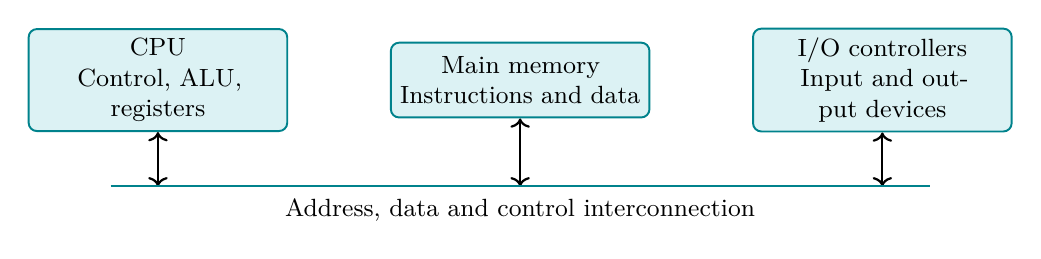
\begin{tikzpicture}[font=\small]
\node[block,text width=3.05cm] (cpu) at (0,0) {CPU\\Control, ALU, registers};
\node[block,text width=3.05cm] (mem) at (4.6,0) {Main memory\\Instructions and data};
\node[block,text width=3.05cm] (io) at (9.2,0) {I/O controllers\\Input and output devices};
\draw[<->,thick] (cpu.south)--(0,-1.35);
\draw[<->,thick] (mem.south)--(4.6,-1.35);
\draw[<->,thick] (io.south)--(9.2,-1.35);
\draw[thick,myteal] (-.6,-1.35)--(9.8,-1.35);
\node[below] at (4.6,-1.38) {Address, data and control interconnection};
\end{tikzpicture}
\end{tcolorbox}

\subsection{Software and program translation}
\begin{itemize}[leftmargin=*,itemsep=3pt]
\item \textbf{Application software} performs a user task. \textbf{System software} includes the operating system, device drivers and language tools. The operating system manages processor time, memory, files and devices.
\item \textbf{Compiler and assembler.} A compiler generally translates high-level source to assembly or object code. An assembler translates mnemonics to machine encodings, resolves local labels and records unresolved addresses for relocation.
\item \textbf{Linker and loader.} A linker combines object files and libraries, resolves symbols and relocates references. A loader maps a program into memory and transfers control to its entry point.
\item \textbf{Performance impact.} Algorithm and compiler change executed instruction count and locality. The operating system can add scheduling, interrupt and I/O time. Compare actual workloads and execution time.
\end{itemize}
\subsection{Execution time, CPI and Amdahl's law}
\begin{tcolorbox}[defbox,title={Latency, throughput and CPI}]
Latency is time for one task. Throughput is work completed per unit time. Cycles per instruction (CPI) is the average number of processor cycles per executed instruction for a workload.
\end{tcolorbox}

For dynamic instruction counts $N_i$ by class, $N=\sum_i N_i$. Count each class's cycles and divide CPU cycles by the clock frequency $f$:
\[
\begin{aligned}
\mathrm{CPI}_{\rm avg}&=\sum_i(N_i/N)\mathrm{CPI}_i,\\
T_{\rm CPU}&=\frac{\sum_i N_i\,\mathrm{CPI}_i}{f}
            =N\,\mathrm{CPI}_{\rm avg}T_{\rm clk},\qquad T_{\rm clk}=1/f .
\end{aligned}
\]
\begin{tcolorbox}[examplebox,title={Compare two implementations on one workload}]
The program executes $60$ million instructions at 1 cycle, $30$ million at 2 cycles, and $10$ million at 5 cycles on machine A.
\[
\begin{aligned}
N&=100\times10^6,\quad
N_{\rm cycles}=(60+60+50)\times10^6,\\
\mathrm{CPI}_A&=1.70,\quad T_A=170\times10^6/(2\times10^9)=85\,\mathrm{ms}.
\end{aligned}
\]
Machine B executes $85$ million instructions at mean CPI 2.4 and $2.4\,\mathrm{GHz}$. $T_B=85\,\mathrm{ms}$ as well. Frequency alone does not determine speed.
\end{tcolorbox}
\begin{itemize}[leftmargin=*,itemsep=3pt]
\item \textbf{Speedup.} Use $T_{\rm old}/T_{\rm new}$ for the same task. Millions of instructions per second (MIPS) equals $f/(10^6\mathrm{CPI})$ when $f$ is in hertz. MIPS can be misleading across instruction sets because each instruction may do a different amount of work.
\item \textbf{Amdahl's law.} If fraction $p$ of the original time runs $s$ times faster, $T_{\rm new}=T_{\rm old}[(1-p)+p/s]$. Overall speedup is $1/[(1-p)+p/s]$. For $p=0.4$ and $s=4$, total speedup is $1/0.7=1.43$, limited to $1/0.6=1.67$ even with unlimited acceleration of that part.
\end{itemize}

\section{Instructions, Addressing and Assembly}
\begin{tcolorbox}[defbox,title={Instruction set architecture}]
An instruction set architecture (ISA) is the hardware--software contract for machine instructions. The opcode identifies the operation. Operand fields identify registers, immediate values or how to locate memory operands.
\end{tcolorbox}
\subsection{Instruction types, formats and instruction cycle}
\begin{itemize}[leftmargin=*,itemsep=3pt]
\item \textbf{Data movement.} Load reads memory to a register. Store writes a register value to memory. Move copies a value, generally without arithmetic.
\item \textbf{Data processing.} Arithmetic, logic, shifts, comparison and bit testing work on operands and may update condition codes.
\item \textbf{Control transfer.} Branch, jump, call and return can replace the sequential next program counter (PC). Conditional branches test a flag or register condition.
\item \textbf{System operations.} System calls, interrupt-return and control-register operations connect application execution with privileged system services.
\end{itemize}
\begin{enumerate}[leftmargin=*,itemsep=3pt]
\item \textbf{Fetch.} Read the instruction addressed by the PC. Compute the sequential successor address (PC plus instruction length).
\item \textbf{Decode.} Interpret the opcode and operand fields. Read registers and form an effective address if required.
\item \textbf{Execute and access memory.} The ALU computes a result, condition or address. An instruction may then read or write data memory.
\item \textbf{Commit architectural effects.} Write destination registers or flags and select the next PC. A branch can override the sequential address.
\end{enumerate}
\par\vspace{6pt}\noindent
\begin{tabularx}{\linewidth}{|B{2.35cm}|Y|Y|}\hline
Format & Example for $X=(A+B)C$ & Where operands are found \\ \hline
Three address & \texttt{ADD T,A,B} then \texttt{MUL X,T,C} & Two explicit inputs and a separate destination. \\ \hline
Two address & \texttt{MOV X,A}, \texttt{ADD X,B}, \texttt{MUL X,C} & One explicit operand is also destination. \\ \hline
One address & \texttt{LOAD A}, \texttt{ADD B}, \texttt{MUL C}, \texttt{STORE X} & Accumulator is implicit. \\ \hline
Zero address & \texttt{PUSH A}, \texttt{PUSH B}, \texttt{ADD}, \texttt{PUSH C}, \texttt{MUL}, \texttt{POP X} & Arithmetic uses the operand stack implicitly. The push/pop instructions can still name addresses. \\ \hline
\end{tabularx}

\begin{tcolorbox}[examplebox,title={Read a toy instruction code}]
Assume a 16-bit format $[\text{opcode:4}][R_d:4][R_s:4][R_t:4]$. If opcode 2 means register addition, hex \texttt{2345} decodes as \texttt{ADD R3,R4,R5}. It writes $R_4+R_5$ into $R_3$. Four opcode bits permit up to 16 primary codes in this format. A different format may use some remaining bits for an immediate or function code.
\end{tcolorbox}
\textbf{ISA styles.} An accumulator ISA uses an implicit accumulator. A stack ISA operates on top-of-stack operands. A general-register ISA may allow register--memory arithmetic or require a load/store model.
\par\vspace{6pt}\noindent
\begin{tabularx}{\linewidth}{|B{2.6cm}|Y|Y|}\hline
Feature & Reduced Instruction Set Computer (RISC) & Complex Instruction Set Computer (CISC) \\ \hline
Encoding & Often uses a small family of regular formats. & Often provides more varied formats and lengths. \\ \hline
Memory operands & Usually explicit loads and stores. Arithmetic operates on registers. & Some arithmetic instructions can directly name a memory operand. \\ \hline
Design effect & Regular operands and encoding can simplify decode and pipelining. & Denser or richer instructions may reduce instruction count, while decode and implementation may need more work. \\ \hline
\end{tabularx}

These are typical design tendencies. Compare CPU time on the same workload because instruction count and implementation both matter.

\subsection{Addressing modes}
Effective address (EA) is the computed memory address of an operand. Let $M[A]$ stand for the contents at address $A$. Assume $R_2=1000$, $R_3=20$, $M[1200]=4000$ and next PC $=2000$.
\par\vspace{6pt}\noindent
\begin{tabularx}{\linewidth}{|B{3.0cm}|Y|Y|}\hline
Mode & Operand or EA rule & Worked reading \\ \hline
Immediate & Literal in instruction & \texttt{\#12} denotes value 12. \\ \hline
Register & Register contents & \texttt{R2} denotes 1000. \\ \hline
Direct & EA is the address field & \texttt{[1200]} reads $M[1200]=4000$. \\ \hline
Memory indirect & EA is the pointer at the address field & Use $M[1200]=4000$ as EA, then read $M[4000]$. \\ \hline
Register indirect & EA is register contents & \texttt{[R2]} reads $M[1000]$. \\ \hline
Base plus displacement & EA is base plus signed constant & \texttt{[R2+16]} has EA $1016$. \\ \hline
Indexed & EA is base plus index, optionally scaled & \texttt{[R2+4*R3]} has EA $1080$. \\ \hline
PC-relative & Branch target is specified PC plus displacement in the chosen units & If relative to next PC and in bytes, $2000-12=1988$. \\ \hline
Auto-increment & Access through a register, then advance it & Word load through $R_2$ with stride 4 uses $1000$ then sets $R_2=1004$. \\ \hline
\end{tabularx}

\subsection{Assembly-language trace}
Assembly instructions typically contain an optional label, mnemonic and operands. A directive guides the assembler, for example to allocate data or place a label. The following illustrative load/store assembly puts the destination operand first.
\begin{tcolorbox}[examplebox,title={Sum three consecutive 32-bit words}]
Start with $R_1=1000$, $R_2=3$, $R_3=0$ and data $7,4,9$ at addresses 1000, 1004, 1008.
\begin{verbatim}
loop: LOAD R4, [R1]
      ADD  R3, R3, R4
      ADDI R1, R1, 4
      SUBI R2, R2, 1
      BNEZ R2, loop
\end{verbatim}
The loaded addresses are 1000, 1004 and 1008. After each iteration $R_3$ is 7, 11 and 20, while $R_2$ is 2, 1 and 0. The branch falls through when the count reaches zero. The address stride is four bytes, not one.
\end{tcolorbox}

\section{Stacks, Queues and Subroutines}
\begin{tcolorbox}[defbox,title={Stack and queue}]
A stack is last-in first-out (LIFO) and supports push/pop at the top. A queue is first-in first-out (FIFO) and inserts at the rear and removes from the front. Stacks support nested calls and expression evaluation. Queues buffer work or data in arrival order.
\end{tcolorbox}

\subsection{Stack convention, calls and returns}
\begin{enumerate}[leftmargin=*,itemsep=2pt]
\item \textbf{Push.} In a full descending stack, subtract word size $w$ from the stack pointer (SP), then write $M[\mathrm{SP}]$. SP points to the top occupied word.
\item \textbf{Pop.} Read $M[\mathrm{SP}]$, then add $w$ to SP. Pushing beyond capacity overflows. Popping an empty stack underflows.
\item \textbf{Call.} Save the next PC in a link register or on the stack, then branch. Save the link before a nested call overwrites it.
\item \textbf{Return.} The calling convention governs arguments, locals and saved registers in the frame. Restore required registers and SP, then load the saved PC.
\end{enumerate}
\begin{tcolorbox}[examplebox,title={Trace a nested call with a downward-growing stack}]
Take $\mathrm{SP}=1000$, $w=4$ and a model that pushes the return address. A call to A saves 104 at 996. A calls B and saves 220 at 992. B returns to 220 and restores $\mathrm{SP}=996$. A returns to 104 and restores $\mathrm{SP}=1000$. Each call unwinds its own frame first.
\end{tcolorbox}
\subsection{Circular hardware queue}
Use $C$ slots with front $h$, next-write position $t$ and occupancy $n$. Enqueue if $n<C$: write at $t$, advance $t$ modulo $C$, and increment $n$. Dequeue if $n>0$: read at $h$, advance $h$ modulo $C$, and decrement $n$. Occupancy distinguishes full from empty when $h=t$. With $C=4$ and both indices at 3, two enqueues use slots 3 and 0.

\newpage
\begin{center}
  {\large\bfseries\color{myred} Quick Revision --- Module 1}\\[3pt]
  {\small\color{mydark} Computer Structure and Instruction Sets $|$ EC502}
\end{center}
\noindent{\color{myred}\rule{\linewidth}{1.2pt}}
\begin{tcolorbox}[formulabox,title={Key Formulas at a Glance}]
\renewcommand{\arraystretch}{1.35}
\begin{tabularx}{\linewidth}{B{5.0cm}Y}
CPU time & $N\cdot\mathrm{CPI}/f$ \\[3pt]
Weighted CPI & $\sum_i(N_i/N)\mathrm{CPI}_i$ \\[3pt]
Amdahl speedup & $1/[(1-p)+p/s]$ \\[3pt]
Scaled index & $\mathrm{EA}=R_b+R_i\cdot\text{scale}+\text{displacement}$ \\[3pt]
Circular index & $\mathrm{next}=(\mathrm{index}+1)\bmod C$ \\[3pt]
\end{tabularx}
\end{tcolorbox}
\begin{tcolorbox}[defbox,title={One-Line Definitions}]
\textbf{Opcode.} Instruction field selecting the operation.\par
\textbf{Effective address.} Address calculated for a memory operand.\par
\textbf{Subroutine.} Callable code that returns control using a saved return address.\par
\end{tcolorbox}
\begin{tcolorbox}[exambox,title={Frequently Asked / Viva Questions}]
\begin{enumerate}[topsep=0pt, label=\textbf{Q\arabic*.}, itemsep=5pt]
\item \Q{What is visible at an ISA boundary?}
Registers, instruction encodings, operations, addressing rules and other programmer-visible state.
\item \Q{Where is the next instruction address held?}
In the program counter.
\item \Q{How do architecture and organisation differ?}
Architecture specifies visible behaviour. Organisation implements it.
\item \Q{What does an assembler produce?}
Encoded machine instructions and, for relocatable objects, symbol and relocation information.
\item \Q{Does a higher clock guarantee lower CPU time?}
Compare instruction count, CPI and frequency together.
\item \Q{What is the difference between immediate and direct addressing?}
Immediate carries the value. Direct carries its memory address.
\item \Q{What distinguishes register indirect from memory indirect?}
The pointer comes from a register in one case and a memory cell in the other.
\item \Q{How can a zero-address add find its operands?}
It takes them from the top of the operand stack.
\item \Q{Why save a return address?}
So the routine can resume the caller at the instruction after the call.
\item \Q{How are a stack and a queue ordered?}
LIFO and FIFO respectively.
\end{enumerate}
\end{tcolorbox}
\begin{tcolorbox}[tikzbox,title={Summary comparison}]
\begin{tabularx}{\linewidth}{|B{4cm}|Y|}\hline
\textbf{Case} & \textbf{What to use} \\ \hline
Instruction fetch & PC selects memory, then the instruction is decoded. \\ \hline
Control transfer & Selects a new PC from a target or saved return address. \\ \hline
Data transfer & Resolve the address first and identify source and destination. \\ \hline
\end{tabularx}
\end{tcolorbox}

% -- Module 2 -----------------------------------------------------------------
\modulestart{2}{Processor Organisation and Data Representation}

\section{Processor Organisation and Data Representation}
\begin{tcolorbox}[defbox,title={Datapath and register-transfer language}]
A datapath is the collection of registers, buses, multiplexers and functional units that hold and transform data. Register-transfer language (RTL) describes operations such as $R_3\leftarrow R_1+R_2$ and the clock events at which registers update.
\end{tcolorbox}
\subsection{Registers, bus structure and flags}
\begin{itemize}[leftmargin=*,itemsep=3pt]
\item \textbf{PC and IR.} The program counter supplies the next instruction address. The instruction register (IR) holds the instruction being decoded or executed in a simple CPU.
\item \textbf{MAR and MDR.} The memory address register (MAR) drives an address. The memory data register (MDR), also called MBR in some models, buffers memory data. In practice these roles may be part of a memory interface rather than named registers.
\item \textbf{General registers and status.} General-purpose registers hold operands and addresses. An accumulator is an implicit operand/result register in an accumulator organisation. Typical status flags are zero $Z$, negative $N$, carry $C$ and signed overflow $V$.
\item \textbf{Internal bus.} On a single bus, select one source driver at a time. Multiple destination registers may latch the same value together. Multiport register files and multiple buses can carry separate inputs and a result in one cycle.
\end{itemize}
\begin{tcolorbox}[tikzbox,title={A three-bus register datapath},unbreakable]
\centering
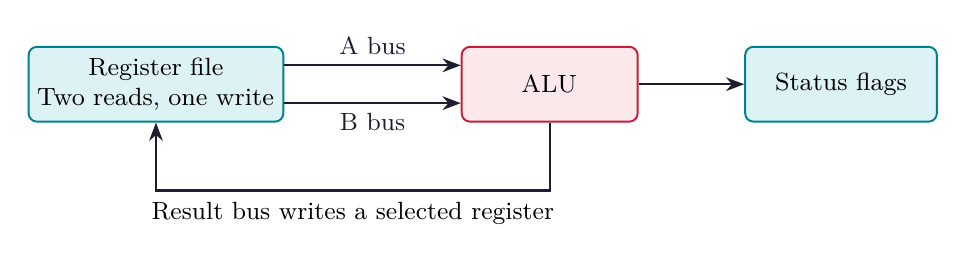
\begin{tikzpicture}[font=\small]
\node[block,text width=3cm] (rf) at (0,0) {Register file\\Two reads, one write};
\node[redblock,text width=2cm] (alu) at (5,0) {ALU};
\node[block,text width=2.2cm] (flags) at (8.7,0) {Status flags};
\draw[arrow] ($(rf.east)+(0,.24)$)--($(alu.west)+(0,.24)$) node[midway,above] {A bus};
\draw[arrow] ($(rf.east)+(0,-.24)$)--($(alu.west)+(0,-.24)$) node[midway,below] {B bus};
\draw[arrow] (alu.east)--(flags.west);
\draw[arrow] (alu.south)--(5,-1.35)--(0,-1.35)--(rf.south);
\node[below] at (2.5,-1.37) {Result bus writes a selected register};
\end{tikzpicture}
\end{tcolorbox}

\begin{tcolorbox}[examplebox,title={One-bus versus three-bus addition}]
For $R_3\leftarrow R_1+R_2$ on a single bus, use temporary registers $Y$ and $Z_{\rm ALU}$.
\begin{enumerate}[leftmargin=*,itemsep=2pt]
\item Place $R_1$ on the bus and latch it in $Y$.
\item Place $R_2$ on the bus, select ADD and latch $Y+R_2$ in $Z_{\rm ALU}$.
\item Place $Z_{\rm ALU}$ on the bus and write $R_3$.
\end{enumerate}
In the illustrated three-bus model, $R_1$ and $R_2$ can be read simultaneously and the result can be written at the clock edge, if the combinational path meets timing.
\end{tcolorbox}

\par\vspace{6pt}\noindent
\begin{tabularx}{\linewidth}{|B{3.2cm}|Y|Y|}\hline
Organisation & Operand and result convention & Trade-off \\ \hline
Accumulator & ALU uses an implicit accumulator and writes it back. & Compact fields, but frequent accumulator spills are possible. \\ \hline
General register & Explicit register fields select operands. & Flexible reuse of values at the cost of more encoding bits and ports. \\ \hline
Stack & ALU removes top entries and pushes one result. & Compact arithmetic encodings. Operand access and data dependence are tied to stack order. \\ \hline
\end{tabularx}

\section{Binary Information and Number Formats}
\subsection{Positional notation, characters and bytes}
\begin{tcolorbox}[defbox,title={Bit, byte and word}]
A bit represents one of two states. A byte has eight bits. A word is a machine-defined unit of data, often 16, 32 or 64 bits. The same pattern can represent an integer, character, instruction or part of an address depending on its interpretation.
\end{tcolorbox}
\begin{itemize}[leftmargin=*,itemsep=3pt]
\item \textbf{Radix.} A digit at position $i$ has weight $b^i$ in radix $b$. For base 2, $(1011.101)_2=8+2+1+1/2+1/8=11.625$.
\item \textbf{Conversion.} Repeatedly divide an integer by the target radix and read remainders in reverse. Repeatedly multiply the fraction by the radix and record each integer part in order. For instance $0.375$ becomes $0.011_2$ because successive products give digits 0, 1, 1.
\item \textbf{Octal and hexadecimal.} Group binary bits in threes for octal or fours for hex, starting at the radix point. Thus $(1101\,0110)_2=\texttt{D6}_{16}$. Pad only the outer ends when needed.
\item \textbf{Binary-coded decimal (BCD).} Encode each decimal digit in four bits. Decimal 59 is \texttt{0101 1001} in 8421 BCD but \texttt{0011 1011} as an unsigned binary integer.
\item \textbf{Character representation.} ASCII assigns codes to 128 basic symbols. Unicode assigns code points and encodings such as UTF-8 store their byte representations. For example, ASCII and UTF-8 both encode \texttt{A} as hex \texttt{41}.
\end{itemize}
\begin{tcolorbox}[examplebox,title={Identify endianness by increasing addresses}]
Store \texttt{0x12345678} as a four-byte word starting at address 100. In big-endian order, addresses 100--103 contain \texttt{12 34 56 78}. In little-endian order, they contain \texttt{78 56 34 12}. Endianness orders bytes in memory. It does not reverse the bits within a byte.
\end{tcolorbox}

\subsection{Signed integers and overflow}
\par\vspace{6pt}\noindent
\begin{tabularx}{\linewidth}{|B{3.5cm}|Y|Y|}\hline
Encoding & For $n$ bits & 8-bit example for $-13$ \\ \hline
Unsigned & $0$ to $2^n-1$. No negative values. & Not representable. \\ \hline
Sign and magnitude & A sign bit and $n-1$ magnitude bits, including two zeros. & \texttt{10001101} \\ \hline
One's complement & Invert all bits of the positive form. Two zeros. & \texttt{11110010} \\ \hline
Two's complement & Invert and add one. Range $-2^{n-1}$ to $2^{n-1}-1$. One zero. & \texttt{11110011} \\ \hline
Biased & Stored unsigned code is value plus a stated bias. & With bias 127, $114=$ \texttt{01110010}. \\ \hline
\end{tabularx}

In two's complement the top bit has weight $-2^{n-1}$. Add or subtract modulo $2^n$, discarding the carry beyond the width. Extend a signed operand by repeating its sign bit. Extend an unsigned operand with zeros. For addition, signed overflow occurs if equal-sign operands yield an opposite-sign result. Equivalently $V=C_{\rm into\ sign}\oplus C_{\rm out\ of\ sign}$. Unsigned addition overflow uses the final carry. For subtraction $A-B$ using $A+\overline B+1$, carry out 1 means no unsigned borrow under this convention.
\begin{tcolorbox}[examplebox,title={Trace signed arithmetic and test the result}]
In eight bits, $+45=\texttt{00101101}$ and $-19=\texttt{11101101}$.
\[
\begin{aligned}
(+45)+(-19)&=\texttt{00101101}+\texttt{11101101}
             =\texttt{00011010}=26,\\
(-45)-(-19)&=\texttt{11010011}+\texttt{00010011}
             =\texttt{11100110}=-26.
\end{aligned}
\]
Both results fit and the first addition's discarded carry does not indicate signed overflow. In four bits $7+3$ gives \texttt{1010}, an invalid signed sum, because two positive operands yielded a negative sign. The same bit pattern correctly encodes unsigned decimal 10.
\end{tcolorbox}

\subsection{Fixed-point and floating-point interpretation}
\begin{itemize}[leftmargin=*,itemsep=4pt]
\item \textbf{Fixed point.} Assign $F$ fractional bits to a stored integer $I$. Its value is $I2^{-F}$, with constant step $2^{-F}$. For an eight-bit signed encoding with $F=4$, range is $-8$ to $7.9375$. The pattern \texttt{11101100} is $I=-20$, hence $-1.25$.
\item \textbf{Fixed-point arithmetic.} Align binary points before addition. The raw product of two values with $F$ fractional bits has $2F$ fractional bits. For a result with $F$ fractional bits, rescale, round and test for overflow.
\item \textbf{Floating point.} Represent a value using sign, significand and an exponent, for example $-1.01_2\times2^3=-10$. Exponents give a larger dynamic range while spacing between adjacent values generally grows with magnitude.
\item \textbf{When to use each.} A known bounded scale can make fixed-point hardware simple and predictable. Floating point accommodates values of widely different sizes, but exponent alignment and rounding add work.
\end{itemize}

\newpage
\begin{center}
  {\large\bfseries\color{myred} Quick Revision --- Module 2}\\[3pt]
  {\small\color{mydark} Processor Organisation and Data Representation $|$ EC502}
\end{center}
\noindent{\color{myred}\rule{\linewidth}{1.2pt}}
\begin{tcolorbox}[formulabox,title={Key Formulas at a Glance}]
\renewcommand{\arraystretch}{1.35}
\begin{tabularx}{\linewidth}{B{5.0cm}Y}
Unsigned range & $0\le x\le 2^n-1$ \\[3pt]
Two's-complement range & $-2^{n-1}\le x\le 2^{n-1}-1$ \\[3pt]
Fixed-point value & $x=I2^{-F}$ with scale $F$ fractional bits \\[3pt]
Signed addition overflow & $V=C_{\rm into\ sign}\oplus C_{\rm out\ of\ sign}$ \\[3pt]
\end{tabularx}
\end{tcolorbox}
\begin{tcolorbox}[defbox,title={One-Line Definitions}]
\textbf{Datapath.} Hardware that stores, routes and transforms operands.\par
\textbf{Sign extension.} Increase two's-complement width by copying the sign bit into the added high positions.\par
\textbf{Endianness.} Order of bytes of a multi-byte value in memory.\par
\end{tcolorbox}
\begin{tcolorbox}[exambox,title={Frequently Asked / Viva Questions}]
\begin{enumerate}[topsep=0pt, label=\textbf{Q\arabic*.}, itemsep=5pt]
\item \Q{What does RTL describe?}
Register transfers and operations scheduled by control signals and clock events.
\item \Q{Why can a single bus not carry two unrelated inputs at once?}
It selects one value source for that transfer.
\item \Q{What is the role of MAR?}
Hold or present the memory transaction address.
\item \Q{How many zeros exist in one's complement?}
Two, the all-zero and all-one patterns.
\item \Q{How is a two's-complement negative obtained?}
Invert the bits and add one within the chosen width.
\item \Q{Can opposite-sign addition overflow in two's complement?}
No, because the integer sum is between the two operands.
\item \Q{What is the carry--borrow convention for the illustrated subtractor?}
Carry out 1 means no unsigned borrow.
\item \Q{Is BCD the same as binary coding of the whole number?}
BCD encodes each decimal digit separately.
\item \Q{Which byte comes first in little-endian memory?}
The least significant byte goes at the lowest address.
\item \Q{Why does floating-point spacing vary?}
Changing the exponent scales the spacing between adjacent significands.
\end{enumerate}
\end{tcolorbox}
\begin{tcolorbox}[tikzbox,title={Summary comparison}]
\begin{tabularx}{\linewidth}{|B{4cm}|Y|}\hline
\textbf{Case} & \textbf{What to use} \\ \hline
MAR / MDR & Address for memory / data going to or from memory. \\ \hline
Fixed point & Constant step and explicitly assigned scale. \\ \hline
Floating point & Significand and exponent trading precision and dynamic range. \\ \hline
\end{tabularx}
\end{tcolorbox}

% -- Module 3 -----------------------------------------------------------------
\modulestart{3}{Computer Arithmetic and ALU Design}

\section{Computer Arithmetic and ALU Design}
\begin{tcolorbox}[defbox,title={Arithmetic logic unit}]
An arithmetic logic unit (ALU) is a combinational circuit that performs selected arithmetic and bitwise operations. An operation field controls the result multiplexer, and flag logic describes the result for later instructions.
\end{tcolorbox}
\subsection{Full adder, ripple carry and carry look-ahead}
For bits $A_i,B_i$ and carry $C_i$, define propagate $P_i=A_i\oplus B_i$ and generate $G_i=A_iB_i$. Then $S_i=P_i\oplus C_i$ and $C_{i+1}=G_i+P_i C_i$, with $+$ denoting Boolean OR in these carry equations.
\begin{itemize}[leftmargin=*,itemsep=3pt]
\item \textbf{Ripple carry.} Chain the full adders. The worst-case carry delay grows with word length because the high stage waits for the low stages.
\item \textbf{Carry look-ahead (CLA).} Substitute the carry recurrence repeatedly. Generate intermediate carries in parallel using the input propagate and generate signals.
\end{itemize}
\[
\begin{aligned}
 C_1&=G_0+P_0C_0,\\
 C_2&=G_1+P_1G_0+P_1P_0C_0,\\
 C_3&=G_2+P_2G_1+P_2P_1G_0+P_2P_1P_0C_0,\\
 C_4&=G_3+P_3G_2+P_3P_2G_1+P_3P_2P_1G_0+P_3P_2P_1P_0C_0 .
\end{aligned}
\]
Define group propagate $P=P_3P_2P_1P_0$ and group generate $G$ as the four $C_4$ terms not multiplying $C_0$. Then $C_4=G+PC_0$. Large adders use groups or a carry tree to limit gate fan-in. The trade-off is extra logic and wiring.
\begin{tcolorbox}[examplebox,title={Trace a carry through a CLA group}]
For $A=\texttt{1011}$, $B=\texttt{0101}$ and $C_0=0$, $P=\texttt{1110}$ and $G=\texttt{0001}$ as bit vectors here. Bit zero generates a carry and the next three bits propagate it. $C_1=C_2=C_3=C_4=1$. The four-bit output is \texttt{0000} with carry out 1.
\end{tcolorbox}

\subsection{Add/subtract, logic and shift selection}
A shared $n$-bit adder uses input $B'_i=B_i\oplus\mathrm{SUB}$ and $C_0=\mathrm{SUB}$. With $\mathrm{SUB}=0$ it adds. With $\mathrm{SUB}=1$ it computes $A+\overline B+1=A-B$ modulo $2^n$.
\begin{tcolorbox}[tikzbox,title={Result selection in a small ALU},unbreakable]
\centering
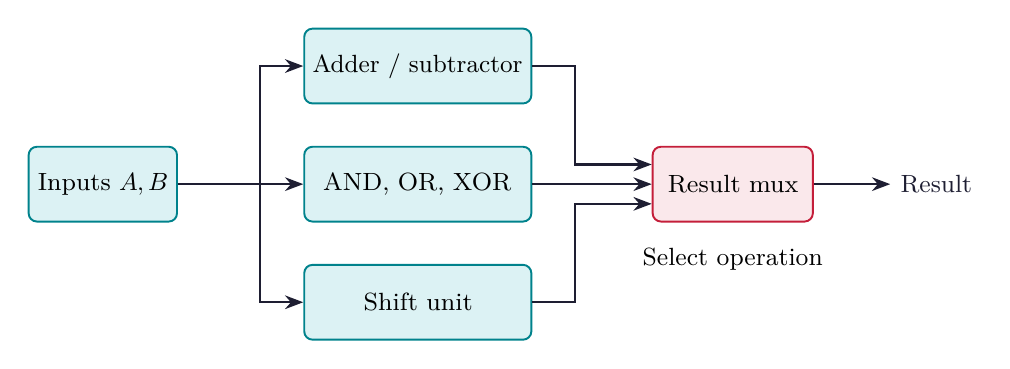
\begin{tikzpicture}[font=\small]
\node[block,text width=1.65cm] (in) at (0,0) {Inputs $A,B$};
\node[block,text width=2.65cm] (arith) at (4,1.5) {Adder / subtractor};
\node[block,text width=2.65cm] (logic) at (4,0) {AND, OR, XOR};
\node[block,text width=2.65cm] (shift) at (4,-1.5) {Shift unit};
\node[redblock,text width=1.8cm] (mux) at (8,0) {Result mux};
\draw[arrow] (in.east)--(2,0)|-(arith.west);
\draw[arrow] (in.east)--(logic.west);
\draw[arrow] (2,0)|-(shift.west);
\draw[arrow] (arith.east)--(6,1.5)|-($(mux.west)+(0,.25)$);
\draw[arrow] (logic.east)--(mux.west);
\draw[arrow] (shift.east)--(6,-1.5)|-($(mux.west)+(0,-.25)$);
\draw[arrow] (mux.east)--(10,0) node[right] {Result};
\node[below] at (8,-.69) {Select operation};
\end{tikzpicture}
\end{tcolorbox}

\begin{itemize}[leftmargin=*,itemsep=3pt]
\item \textbf{Flags.} $Z=1$ when all result bits are zero. $N$ copies the top bit. For add/subtract, carry comes from the top adder position, and signed overflow is the XOR of the carries into and out of that position.
\item \textbf{Shifts.} Logical right shift fills with zero. Arithmetic right shift replicates the sign. Rotate recirculates bits. A barrel shifter selects shifts by powers of two in successive mux stages.
\item \textbf{Compare.} A compare can compute a subtraction only for flags. For conventional two's-complement subtraction, signed less-than uses $N\oplus V$. Unsigned less-than uses borrow, accounted for by the selected carry convention.
\end{itemize}

\section{Binary Multiplication and Division}
\subsection{Unsigned shift-and-add multiplication}
Each bit of the multiplier selects a shifted copy of the multiplicand. For $M=13=\texttt{1101}$ and $Q=11=\texttt{1011}$, the selected copies are $13$, $13\cdot2$ and $13\cdot8$, giving 143 or \texttt{10001111}.
\begin{itemize}[leftmargin=*,itemsep=3pt]
\item \textbf{Sequential multiplier.} Put the multiplier in $Q$ and clear the high accumulator $A$. For each bit, conditionally add $M$ to $A$ when $Q_0=1$, then shift the carry and the joined $A:Q$ right. Keep the extra carry during the shift. After $n$ iterations, $A:Q$ holds the $2n$-bit product.
\item \textbf{Parallel multiplier.} An AND array generates partial products. Carry-save adders reduce rows to two without propagating carry across the entire width at every layer. A final carry-propagate adder adds the two rows. An array or tree costs more hardware than a reused sequential adder.
\end{itemize}

\subsection{Booth signed multiplication}
In radix-2 Booth multiplication, examine $(Q_0,Q_{-1})$, starting with $Q_{-1}=0$. The signed digit at bit $i$ is $q_{i-1}-q_i$. This replaces a run of ones from $i=l$ through $h$ by $2^{h+1}-2^l$ for a run that ends before the sign bit. The sign bit is handled by the same two's-complement recoding. Add $M$ for pair 01, subtract $M$ for 10, and do nothing for 00 or 11. Then arithmetic-right-shift $A:Q:Q_{-1}$ as one unit.
\begin{tcolorbox}[examplebox,title={Booth table for two negative numbers}]
Use $M=-6=\texttt{1010}$, $Q=-3=\texttt{1101}$ and $A=\texttt{0000}$. Use four iterations. The table shows registers after each arithmetic shift.
\par\vspace{6pt}\noindent
\begin{tabularx}{\linewidth}{|B{1.0cm}|B{1.2cm}|Y|B{1.7cm}|B{1.7cm}|B{1.2cm}|}\hline
Step & Pair & Operation before shift & $A$ & $Q$ & $Q_{-1}$ \\ \hline
1 & 10 & $A\leftarrow A-M$ & \texttt{0011} & \texttt{0110} & 1 \\ \hline
2 & 01 & $A\leftarrow A+M$ & \texttt{1110} & \texttt{1011} & 0 \\ \hline
3 & 10 & $A\leftarrow A-M$ & \texttt{0010} & \texttt{0101} & 1 \\ \hline
4 & 11 & No addition & \texttt{0001} & \texttt{0010} & 1 \\ \hline
\end{tabularx}

The joined result is \texttt{00010010}, or $+18$. For a fully general $n$-bit implementation use an extra sign bit in $A$ and sign-extend $M$ before add/subtract, then retain the low $2n$ product bits. This avoids overflow when negating the most negative multiplicand.
\end{tcolorbox}

\subsection{Restoring and non-restoring division}
\begin{tcolorbox}[defbox,title={Division invariant}]
For unsigned dividend $D$ and positive divisor $M$, return quotient $Q$ and remainder $R$ satisfying $D=MQ+R$ and $0\le R<M$. A zero divisor must be detected separately.
\end{tcolorbox}

In register division, initialise $A=0$ and $Q=D$. Repeat $n$ times for an $n$-bit dividend. $A$ is the signed partial remainder and needs enough extra width for the shift and trial addition/subtraction.
\begin{itemize}[leftmargin=*,itemsep=3pt]
\item \textbf{Restoring.} Shift $A:Q$ left, then subtract $M$ from $A$. If the trial is negative, set $Q_0=0$ and add $M$ back. Otherwise set $Q_0=1$.
\item \textbf{Non-restoring.} Remember the sign of $A$ before shift. Shift $A:Q$ left, subtract $M$ if the old sign was nonnegative, otherwise add $M$. Set $Q_0$ to 1 iff the new $A$ is nonnegative. At the end add $M$ once if $A<0$.
\item \textbf{Why the addition works.} If a trial is $A_{\rm trial}=a-M<0$, restoring then taking the next trial with incoming bit $b$ would give $2a+b-M$. Non-restoring obtains the same quantity as $2(a-M)+b+M$.
\end{itemize}
\begin{tcolorbox}[examplebox,title={Restoring and non-restoring traces for 13 divided by 3}]
Use $Q=\texttt{1101}$ and $M=3$. The quotient register in the last column is common to both runs at each step.
\par\vspace{6pt}\noindent
\begin{tabularx}{\linewidth}{|B{1.1cm}|Y|Y|Y|B{1.6cm}|}\hline
Step & Restoring trial & After restoration if needed & Non-restoring new $A$ & $Q$ \\ \hline
1 & $-2$ & $1$ & $-2$ & \texttt{1010} \\ \hline
2 & $0$ & $0$ & $0$ & \texttt{0101} \\ \hline
3 & $-3$ & $0$ & $-3$ & \texttt{1010} \\ \hline
4 & $-2$ & $1$ & $-2$ & \texttt{0100} \\ \hline
\end{tabularx}

The non-restoring method corrects $-2$ to $1$ at the end. In each case $Q=4$, $R=1$, and $13=3(4)+1$. Signed division can divide magnitudes and then apply the quotient and remainder sign convention. A minimum signed integer divided by $-1$ can overflow at fixed width.
\end{tcolorbox}

\section{IEEE 754 Formats and Floating-Point Arithmetic}
\subsection{Stored fields and special cases}
\begin{tcolorbox}[defbox,title={Binary floating-point format}]
An IEEE 754 binary interchange value uses a sign bit $s$, a biased exponent field $e$, and a fraction field of $p$ bits. Interpret the fields using the exponent class before applying the value formula.
\end{tcolorbox}
\par\vspace{6pt}\noindent
\begin{tabularx}{\linewidth}{|B{3cm}|Y|Y|Y|}\hline
Format & Sign / exponent / fraction & Bias & Normal precision \\ \hline
Binary32 & $1/8/23$ & $127$ & $24$ bits \\ \hline
Binary64 & $1/11/52$ & $1023$ & $53$ bits \\ \hline
\end{tabularx}

Let $F$ be the unsigned integer encoded by the fraction bits and $f=F/2^p$. With all-ones exponent denoted $e_{\max}$:
\begin{itemize}[leftmargin=*,itemsep=3pt]
\item \textbf{Normal} ($0<e<e_{\max}$): $(-1)^s(1+f)2^{e-\mathrm{bias}}$. The leading 1 is implicit.
\item \textbf{Subnormal} ($e=0,\ F\ne0$): $(-1)^s f2^{1-\mathrm{bias}}$. The hidden bit is 0. Smallest positive binary32 normal is $2^{-126}$ and smallest subnormal is $2^{-149}$.
\item \textbf{Signed zero} ($e=0,\ F=0$): $\pm0$. \textbf{Infinity} ($e=e_{\max},\ F=0$): $\pm\infty$. \textbf{NaN} ($e=e_{\max},\ F\ne0$): not a number, as can result from $0/0$.
\end{itemize}
\begin{tcolorbox}[examplebox,title={Encode negative 13.25 in binary32}]
Magnitude $13.25=1101.01_2=1.10101_2\times2^3$. Set $s=1$ and $e=3+127=130=\texttt{10000010}$. Store fraction bits \texttt{10101} followed by 18 zeros. Concatenating fields gives hexadecimal \texttt{C1540000}. To decode it, restore the leading 1, subtract the bias and apply the sign.
\end{tcolorbox}

\subsection{Addition, subtraction, multiplication and division}
\begin{enumerate}[leftmargin=*,itemsep=3pt]
\item \textbf{Unpack and classify.} Separate signs, exponents and significands. Handle zeros, infinities and NaNs as specified before using normal-number formulas.
\item \textbf{Add or subtract.} Align exponents by shifting the smaller-exponent significand right. Add or subtract according to the signs. Normalise the result and update the exponent. Cancellation may require left shifts. Example:
\[
 (1.101_2\times2^3)+(1.1_2\times2^0)
 =(1.101_2+0.0011_2)2^3=1.1101_2\times2^3 .
\]
\item \textbf{Multiply or divide.} XOR the signs. Multiply significands and add unbiased exponents, or divide significands and subtract unbiased exponents. Normalise afterwards. For multiplication, $(1.1_2\times2^0)(1.1_2\times2^{-1})=10.01_2\times2^{-1}=1.001_2\times2^0$.
\item \textbf{Round and pack.} Round to the target precision and range, then pack the fields. Rounding can create a new carry and change the exponent.
\end{enumerate}
\begin{tcolorbox}[examplebox,title={Normalise after subtraction and division}]
\[
\begin{aligned}
(1.010_2-1.001_2)2^2
 &=0.001_2\times2^2=1.000_2\times2^{-1},\\
\frac{1.001_2\times2^3}{1.1_2\times2^1}
 &=0.11_2\times2^2=1.1_2\times2^1 .
\end{aligned}
\]
The subtraction cancels leading bits and requires three left shifts. The division yields a significand below one and requires one left shift. Decrease the exponent once per left shift.
\end{tcolorbox}

\subsection{Rounding and exceptions}
\begin{itemize}[leftmargin=*,itemsep=3pt]
\item \textbf{Guard, round and sticky.} The first two extra bits are guard and round. Sticky is the OR of the remaining discarded bits.
\item \textbf{Nearest, ties-to-even.} Increment the retained significand if guard is 1 and any of round, sticky or the last retained bit is 1. At a midpoint select the even last bit. With three fraction bits, $1.0101000_2$ rounds to $1.010_2$ and $1.0111000_2$ rounds to $1.100_2$.
\item \textbf{Other rounding directions.} Directed modes can round toward zero, $+\infty$ or $-\infty$.
\item \textbf{Status conditions.} Invalid operation, division by zero, overflow, underflow and inexact result are distinct. Overflow handling depends on the rounding direction. Subnormals allow gradual underflow. An exactly representable subnormal does not by itself imply inexact underflow.
\end{itemize}

\newpage
\begin{center}
  {\large\bfseries\color{myred} Quick Revision --- Module 3}\\[3pt]
  {\small\color{mydark} Computer Arithmetic and ALU Design $|$ EC502}
\end{center}
\noindent{\color{myred}\rule{\linewidth}{1.2pt}}
\begin{tcolorbox}[formulabox,title={Key Formulas at a Glance}]
\renewcommand{\arraystretch}{1.35}
\begin{tabularx}{\linewidth}{B{5.0cm}Y}
Full-adder carry & $C_{i+1}=G_i+P_i C_i$ \\[3pt]
Shared add/subtract & $B'=B\oplus\mathrm{SUB}$ and $C_0=\mathrm{SUB}$ \\[3pt]
Booth pair rule & 01 adds, 10 subtracts, 00 and 11 hold \\[3pt]
Unsigned division & $D=MQ+R$ with $0\le R<M$ \\[3pt]
IEEE normal & $(-1)^s(1+f)2^{e-\mathrm{bias}}$ \\[3pt]
IEEE subnormal & $(-1)^sf2^{1-\mathrm{bias}}$ \\[3pt]
\end{tabularx}
\end{tcolorbox}
\begin{tcolorbox}[defbox,title={One-Line Definitions}]
\textbf{Generate bit.} Indicates an output carry independent of the incoming carry.\par
\textbf{Sticky bit.} OR of the bits discarded beyond the round bit.\par
\textbf{Subnormal.} Nonzero floating-point value with a zero exponent field and an implicit leading zero.\par
\end{tcolorbox}
\begin{tcolorbox}[exambox,title={Frequently Asked / Viva Questions}]
\begin{enumerate}[topsep=0pt, label=\textbf{Q\arabic*.}, itemsep=5pt]
\item \Q{Why is ripple carry slow at large widths?}
A carry may propagate through all stages.
\item \Q{Why does subtract set carry-in to one?}
It completes the two's complement of the second operand.
\item \Q{How many product bits suffice for two n-bit inputs?}
A full-width product uses $2n$ bits.
\item \Q{Which shift follows each Booth action?}
An arithmetic right shift of the joined accumulator, multiplier and saved bit.
\item \Q{What is restored in restoring division?}
A negative trial partial remainder is returned to its value before subtraction.
\item \Q{What is the final correction in non-restoring division?}
Add the divisor once if the final remainder is negative.
\item \Q{Why align exponents before floating-point addition?}
Significands must use the same power-of-two scale.
\item \Q{How many stored fraction bits does binary64 use?}
52, giving 53 bits of normal precision.
\item \Q{What distinguishes infinity from NaN?}
With all-ones exponent, infinity has zero fraction and NaN has nonzero fraction.
\item \Q{What does ties-to-even do at an exact midpoint?}
Selects the result whose last retained significand bit is zero.
\end{enumerate}
\end{tcolorbox}
\begin{tcolorbox}[tikzbox,title={Summary comparison}]
\begin{tabularx}{\linewidth}{|B{4cm}|Y|}\hline
\textbf{Case} & \textbf{What to use} \\ \hline
Ripple / CLA & Serial carry propagation / parallel group carry equations. \\ \hline
Restoring / non-restoring & Correct negative trials immediately / compensate in the next cycle and correct at the end. \\ \hline
Normal / subnormal & Implicit leading one / implicit leading zero. \\ \hline
\end{tabularx}
\end{tcolorbox}

% -- Module 4 -----------------------------------------------------------------
\modulestart{4}{Hardwired and Microprogrammed Control}

\section{Hardwired and Microprogrammed Control}
\begin{tcolorbox}[defbox,title={Control unit and instruction interpretation}]
The control unit converts a machine instruction into an ordered sequence of datapath and memory actions. An instruction is the ISA operation visible to software. A micro-operation is an internal register transfer, ALU operation, shift or similar step implementing it.
\end{tcolorbox}
\subsection{Instruction sequencing on a single bus}
Assume byte addresses, four-byte instructions, a single internal bus, an ALU input latch $Y$, an ALU result latch $Z_{\rm ALU}$ and an independent memory data path to the MDR. A memory-ready signal means read data can now be latched. Transfers on the internal bus and independent local operations may share a cycle only if their signals do not conflict.
\par\vspace{6pt}\noindent
\begin{tabularx}{\linewidth}{|B{2.5cm}|Y|Y|}\hline
Phase & Register transfers & Decision or completion \\ \hline
$F_0$ & $\mathrm{MAR}\leftarrow\mathrm{PC}$ and $Z_{\rm ALU}\leftarrow\mathrm{PC}+4$ from the same bus value using a constant ALU input. & Prepare read and sequential PC. \\ \hline
$F_1$ & $\mathrm{PC}\leftarrow Z_{\rm ALU}$ and request instruction read through MAR. & Hold request until memory ready. MDR latches read data on the ready edge. Rewriting the same PC while waiting is harmless in this model. \\ \hline
$F_2$ & $\mathrm{IR}\leftarrow\mathrm{MDR}$. & The instruction is now available to decode. \\ \hline
Decode & Test opcode and addressing mode. & Dispatch to the corresponding execution routine or state. \\ \hline
$A_0,A_1,A_2$ & For \texttt{ADD R3,R1,R2}: $Y\leftarrow R_1$, then $Z_{\rm ALU}\leftarrow Y+R_2$, then $R_3\leftarrow Z_{\rm ALU}$. & Update flags as specified by the ISA. Return to fetch unless another event is accepted. \\ \hline
\end{tabularx}

\begin{itemize}[leftmargin=*,itemsep=3pt]
\item \textbf{Memory operand.} Compute the effective address, load MAR, issue read, wait, and route MDR to the ALU or a destination. A memory-indirect addressing mode first reads a pointer and uses that pointer for a second memory access.
\item \textbf{Branch.} For a taken PC-relative branch in this model, add the sign-extended, correctly scaled displacement to the sequential PC. Select this target instead of the sequential address.
\item \textbf{Interrupt.} At an instruction boundary in a simple precise model, save the resume PC and required status, then select a handler address. Interrupt return restores the state needed to resume.
\end{itemize}

\subsection{Design a hardwired CPU controller}
\begin{tcolorbox}[defbox,title={Hardwired control}]
A hardwired controller generates control signals using a finite-state machine (FSM) and logic gates or programmable logic. Combinational logic decodes state, opcode and conditions. State registers hold the current step.
\end{tcolorbox}

\begin{enumerate}[leftmargin=*,itemsep=3pt]
\item \textbf{List operations.} Write the required RTL first. Separate any transfers that compete for the bus or depend on data produced only at an edge.
\item \textbf{Choose states and transitions.} Use a fixed sequence counter and decoded timing pulses for simple straight-line sequences. Use an FSM for variable paths involving memory wait, condition flags or instruction-dependent cycle counts.
\item \textbf{Write outputs.} A Moore output depends on state; a Mealy output can also depend on current inputs. For the fetch above, assert \texttt{PCout} in $F_0$, \texttt{IRin} in $F_2$, and read request in $F_1$. Assert MDR latch enable when $F_1$ and ready are both true.
\item \textbf{Implement and check.} Encode states using binary or one-hot encoding, derive next-state and output logic, and implement with gates, decoders or a programmable logic array (PLA). Check reset, memory wait, branch conditions, and mutual exclusion of bus drivers.
\end{enumerate}
\begin{tcolorbox}[tikzbox,title={Hardwired control inputs, state and outputs},unbreakable]
\centering
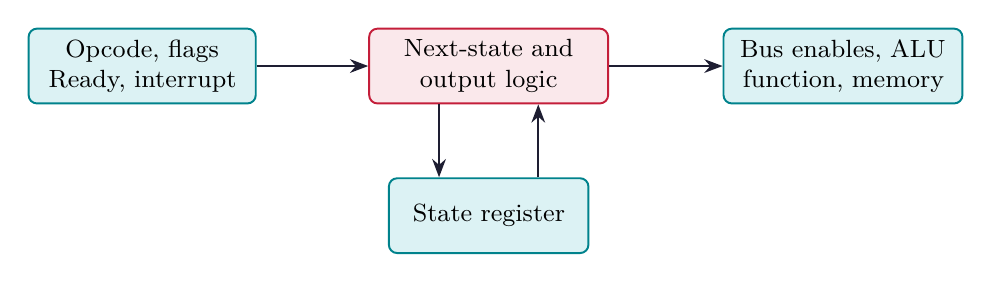
\begin{tikzpicture}[font=\small]
\node[block,text width=2.65cm] (i) at (0,0) {Opcode, flags\\Ready, interrupt};
\node[redblock,text width=2.8cm] (l) at (4.4,0) {Next-state and\\output logic};
\node[block,text width=2.8cm] (o) at (8.9,0) {Bus enables, ALU\\function, memory};
\node[block,text width=2.3cm] (s) at (4.4,-1.9) {State register};
\draw[arrow] (i.east)--(l.west);
\draw[arrow] (l.east)--(o.west);
\draw[arrow] ($(l.south)+(-.63,0)$)--($(s.north)+(-.63,0)$);
\draw[arrow] ($(s.north)+(.63,0)$)--($(l.south)+(.63,0)$);
\end{tikzpicture}
\end{tcolorbox}

\begin{tcolorbox}[examplebox,title={Derive a state equation with a memory wait}]
Use one-hot state bits $F_0,F_1,F_2$ and ready input $M$. Fetch enters $F_1$ from $F_0$. It stays there while not ready, and enters $F_2$ on ready.
\[
 F_1^{+}=F_0+F_1\overline M,\qquad
 F_2^{+}=F_1M,\qquad
 \mathrm{MDRin}=F_1M .
\]
Here $+$ is Boolean OR and superscript $+$ denotes the next stored state. In a one-hot design the reset path establishes one valid starting state. Require the readiness input to obey the interface timing or synchronise it before use.
\end{tcolorbox}

\section{Microprogrammed CPU Control}
\begin{tcolorbox}[defbox,title={Microinstruction and control store}]
A microinstruction holds control actions for a microcycle and information used to choose the next microaddress. A microprogram in a control store implements an ISA instruction or a shared routine such as fetch. The micro-PC addresses the control store, while the ISA PC addresses program memory.
\end{tcolorbox}

\begin{tcolorbox}[tikzbox,title={Microprogrammed controller},unbreakable]
\centering
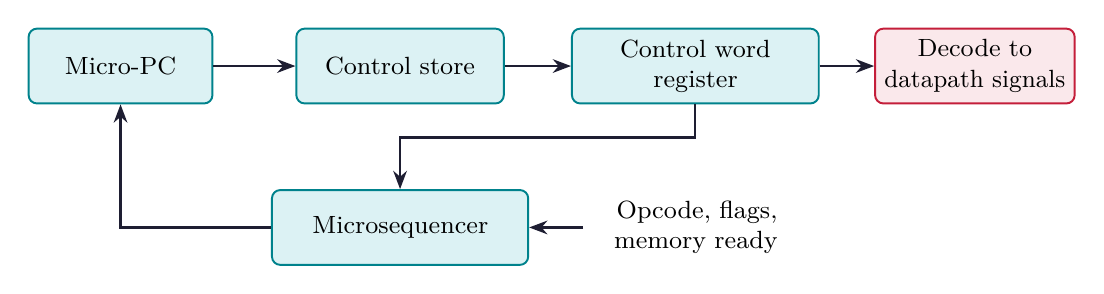
\begin{tikzpicture}[font=\small]
\node[block,text width=2.1cm] (pc) at (0,0) {Micro-PC};
\node[block,text width=2.4cm] (store) at (3.55,0) {Control store};
\node[block,text width=2.90cm] (mir) at (7.3,0) {Control word\\register};
\node[redblock,text width=2.3cm] (out) at (10.85,0) {Decode to\\datapath signals};
\node[block,text width=3.02cm] (seq) at (3.55,-2.05) {Microsequencer};
\node[align=center,text width=2.6cm] (cond) at (7.3,-2.05) {Opcode, flags,\\memory ready};
\draw[arrow] (pc.east)--(store.west);
\draw[arrow] (store.east)--(mir.west);
\draw[arrow] (mir.east)--(out.west);
\draw[arrow] (mir.south)--++(0,-.42)-|(seq.north);
\draw[arrow] (cond.west)--(seq.east);
\draw[arrow] (seq.west)-|(pc.south);
\end{tikzpicture}
\end{tcolorbox}

\subsection{Sequencer, dispatch and example microprogram}
\begin{itemize}[leftmargin=*,itemsep=3pt]
\item \textbf{Fetch microinstruction.} Address the control store with the micro-PC and latch the control word in the microinstruction register (MIR), where the design uses a separate latch.
\item \textbf{Execute micro-operations.} Direct signal bits or decoded fields select register enables, ALU operation and memory controls.
\item \textbf{Select next address.} Choose increment, explicit target, conditional target, opcode dispatch or return from a shared microsubroutine. Opcode mapping supplies an entry address, not a complete execution sequence. Flags may select one of two targets.
\end{itemize}
\par\vspace{6pt}\noindent
\begin{tabularx}{\linewidth}{|B{1.7cm}|Y|Y|}\hline
Address & Control action in the model above & Next address \\ \hline
0 & Perform $F_0$. & 1 \\ \hline
1 & Perform $F_1$, latch MDR only on ready. & If ready then 2, otherwise 1. \\ \hline
2 & Perform $F_2$. & 3 \\ \hline
3 & Decode and dispatch by opcode. & For ADD go to 16, for other operations use their entry points. \\ \hline
16--18 & Schedule $A_0,A_1,A_2$ in order. & Increment through the routine, then jump to 0. \\ \hline
\end{tabularx}

\subsection{Minimise microinstruction size}
\begin{itemize}[leftmargin=*,itemsep=3pt]
\item \textbf{Horizontal.} Allot one bit per independent control line. Wide words can express parallel actions directly and need little control-field decoding.
\item \textbf{Vertical or field encoded.} Encode mutually exclusive actions in a field. Decode the field to select one of them. Separate fields preserve parallelism across groups. Include a no-operation encoding if that group may be idle.
\item \textbf{Sequencing reductions.} Use implicit next-address increment for ordinary steps, reusable micro-routines, and optional branch formats where appropriate. Count address and condition bits explicitly. A $W$-word store needs $\lceil\log_2W\rceil$ address bits.
\end{itemize}
\begin{tcolorbox}[examplebox,title={Compute control-store width}]
Assume eight mutually exclusive source enables, five mutually exclusive ALU functions, and six independent enables. Direct control needs $8+5+6=19$ control bits. Encoding source and ALU with an idle choice needs $\lceil\log_2 9\rceil+\lceil\log_2 6\rceil+6=13$ bits. For a 256-word store with a full next-address field and 2 sequencing bits per word, total width falls from $19+8+2=29$ to $13+8+2=23$ bits. This saves $6(256)=1536$ store bits at the cost of field decoding.
\end{tcolorbox}

\section{Multiplier Control Unit}
\begin{tcolorbox}[defbox,title={Sequential multiplier controller}]
The multiplier controller schedules load, conditional add, shift, decrement and completion. Its status inputs include the multiplier's low bit and the counter-zero condition.
\end{tcolorbox}

For unsigned $n$-bit operands, place the multiplicand in $M$ and the multiplier in $Q$. The accumulator is $A$ and $C$ keeps carry. Use separate states for add and shift to preserve carry. The same state table can drive hardwired gates or a microprogram.
\par\vspace{6pt}\noindent
\begin{tabularx}{\linewidth}{|B{2.6cm}|Y|Y|}\hline
State & Datapath action & Transition \\ \hline
LOAD & Clear $C,A$. Load $M,Q$ and count $n$. & TEST \\ \hline
TEST & Inspect $Q_0$. & If 1, go to ADD. Otherwise go to SHIFT. \\ \hline
ADD & $(C,A)\leftarrow A+M$ using the carry output. & SHIFT \\ \hline
SHIFT & Logical-right-shift $C:A:Q$ and decrement the count. The shifted-in bit at the top is zero. & If the post-decrement count is zero, go to DONE. Otherwise TEST. In a synchronous design test pre-decrement count $=1$ to make this choice at the same edge. \\ \hline
DONE & Assert completion. Read product from $A:Q$. & Idle or LOAD for a new request. \\ \hline
\end{tabularx}

\textbf{Trace.} For $n=3$, $M=3$ and $Q=5$, the three post-shift pairs $(A,Q)$ are $(1,6)$, $(0,7)$ and $(1,7)$. The product is $1\cdot2^3+7=15$. The shifting and count continue even on the iteration that skips ADD.

\newpage
\begin{center}
  {\large\bfseries\color{myred} Quick Revision --- Module 4}\\[3pt]
  {\small\color{mydark} Hardwired and Microprogrammed Control $|$ EC502}
\end{center}
\noindent{\color{myred}\rule{\linewidth}{1.2pt}}
\begin{tcolorbox}[formulabox,title={Key Formulas at a Glance}]
\renewcommand{\arraystretch}{1.35}
\begin{tabularx}{\linewidth}{B{5.0cm}Y}
Fetch address & $\mathrm{MAR}\leftarrow\mathrm{PC}$ \\[3pt]
Simple wait loop & $F_1^{+}=F_0+F_1\overline M$ \\[3pt]
Encoded group & $\lceil\log_2(k+1)\rceil$ bits for $k$ actions plus idle \\[3pt]
Store capacity & Microinstruction width times depth, in bits \\[3pt]
Multiplier termination & Initial count $n$, decrement once per shift \\[3pt]
\end{tabularx}
\end{tcolorbox}
\begin{tcolorbox}[defbox,title={One-Line Definitions}]
\textbf{Micro-operation.} Elementary internal data transfer or computation.\par
\textbf{Control store.} Memory holding the routines that generate CPU control signals.\par
\textbf{Opcode dispatch.} Selection of a microprogram or controller entry state from an opcode.\par
\end{tcolorbox}
\begin{tcolorbox}[exambox,title={Frequently Asked / Viva Questions}]
\begin{enumerate}[topsep=0pt, label=\textbf{Q\arabic*.}, itemsep=5pt]
\item \Q{What is instruction interpretation in a control unit?}
Decoding the instruction and generating the steps that implement its specified operation.
\item \Q{What is the difference between PC and micro-PC?}
PC locates the machine instruction. Micro-PC locates a control-store entry.
\item \Q{Why hold a memory request until ready in this model?}
A fixed cycle count cannot guarantee that memory has produced valid data.
\item \Q{Can two registers drive a single internal bus together?}
The controller normally enables exactly one driver per transfer.
\item \Q{Where do hardwired outputs come from?}
Logic using timing or FSM state, opcode and relevant inputs.
\item \Q{How does a microsequencer handle branches?}
It selects among increment, target, dispatch or return using the microinstruction and conditions.
\item \Q{Where does field encoding save bits?}
Within sets of mutually exclusive actions.
\item \Q{What does a horizontal control word favour?}
Direct selection of many concurrent micro-operations.
\item \Q{When does an unsigned multiplier add the multiplicand?}
When the current low multiplier bit is one.
\item \Q{Why preserve the carry in a multiplier shift?}
It is the high bit of the partial sum and shifts into the accumulator.
\end{enumerate}
\end{tcolorbox}
\begin{tcolorbox}[tikzbox,title={Summary comparison}]
\begin{tabularx}{\linewidth}{|B{4cm}|Y|}\hline
\textbf{Case} & \textbf{What to use} \\ \hline
Hardwired & Control logic implements sequencing directly. Changes can require logic redesign. \\ \hline
Microprogrammed & Control store and sequencer implement steps. Changes can be made in a writable or replaceable store. \\ \hline
Hybrid & Fast common operations may use direct logic, with microcode for more complex sequences. \\ \hline
\end{tabularx}
\end{tcolorbox}

% -- Module 5 -----------------------------------------------------------------
\modulestart{5}{Memory Organisation and Virtual Memory}

\section{Memory Organisation and Virtual Memory}
\begin{tcolorbox}[defbox,title={Memory hierarchy}]
A memory hierarchy places small fast storage near the processor and larger slower storage farther away. Recent reuse (temporal locality) and access to nearby addresses (spatial locality) help a small upper level serve many references.
\end{tcolorbox}
\begin{tcolorbox}[tikzbox,title={Hierarchy and the direction of the trade-off},unbreakable]
\centering
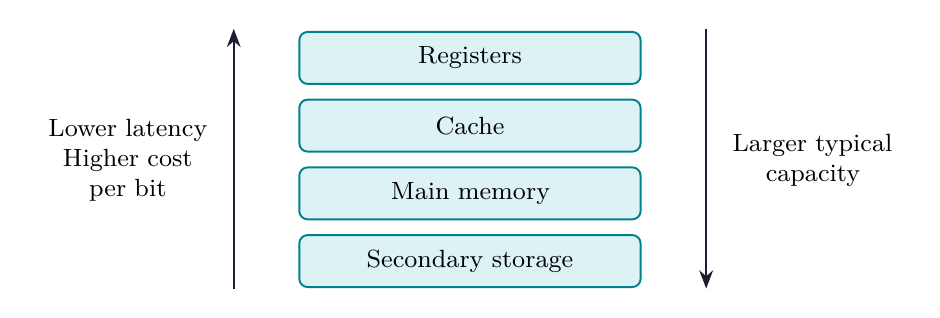
\begin{tikzpicture}[font=\small]
\foreach \y/\name in {0/Registers,-.86/Cache,-1.72/Main memory,-2.58/Secondary storage}{
 \node[block,text width=4.1cm,minimum height=.66cm] at (0,\y) {\name};
}
\draw[arrow] (-3,-2.93)--(-3,.37);
\node[align=center,text width=2.3cm] at (-4.35,-1.3) {Lower latency\\Higher cost per bit};
\draw[arrow] (3,.37)--(3,-2.93);
\node[align=center,text width=2.3cm] at (4.35,-1.3) {Larger typical\\capacity};
\end{tikzpicture}
\end{tcolorbox}

\subsection{Device characteristics and chip organisation}
\begin{itemize}[leftmargin=*,itemsep=3pt]
\item \textbf{Capacity.} A memory of $2^a$ words, each $w$ bits wide, stores $2^aw$ bits. It needs $a$ logical word-address bits. Physical pins may multiplex row and column addresses.
\item \textbf{Latency and cycle time.} Access time is the delay from request to usable data. Cycle time is the minimum interval between suitable successive operations. Transfer bandwidth is bits or bytes transferred per unit time. Burst access can have a high first-word latency but good bandwidth.
\item \textbf{Volatility and endurance.} Volatile devices lose data without power. Nonvolatile devices retain it. Some nonvolatile devices have erase-block constraints and finite program/erase endurance.
\item \textbf{Control and banks.} Chip select enables one chip group. Read/write or output-enable signals control the transfer. With low-order interleaving, word $A$ goes to bank $A\bmod B$ and row $\lfloor A/B\rfloor$ for $B$ banks. Consecutive accesses can overlap if controllers and banks permit.
\end{itemize}
\begin{tcolorbox}[examplebox,title={Build a wider and deeper memory}]
Build $16\mathrm{K}\times16$ from $4\mathrm{K}\times8$ chips, with $\mathrm K=1024$.
\begin{enumerate}[leftmargin=*,itemsep=2pt]
\item Width: two chips in parallel share the address and control signals. One supplies each byte.
\item Depth: four banks of two chips give $16\mathrm K$ word addresses, using eight chips total.
\item Decode: 12 low word-address bits go to every chip. Two high word-address bits select one bank. The total data width is 16 bits. In a byte-addressed host, one additional low address bit selects the byte within a word.
\end{enumerate}
\end{tcolorbox}

\subsection{RAM, ROM and memory technologies}
Random-access memory (RAM) supports read/write access by address. Read-only memory (ROM) families retain data without power and differ in how they can be programmed.
\par\vspace{6pt}\noindent
\begin{tabularx}{\linewidth}{|B{3cm}|Y|Y|}\hline
Device & Storage and operation & Common role \\ \hline
Static RAM (SRAM) & A typical CMOS cell uses six transistors in a latch and access path. State persists while powered without refresh. & Fast but less dense. Common in caches and small on-chip memories. \\ \hline
Dynamic RAM (DRAM) & A typical cell uses one transistor and one capacitor. Charge leaks, so refresh is required. Sense amplifiers restore data after reading. Row activation opens a row buffer. & Dense, volatile main memory. Row hits can be faster than opening a different row. \\ \hline
Synchronous DRAM (SDRAM) & DRAM commands and transfers are coordinated by a clocked interface. A burst can transfer several words per command. Double-data-rate (DDR) families transfer data on both clock edges. & Main memory. Synchronous timing describes the interface, not a different basic bit cell. \\ \hline
Mask ROM / PROM & Mask ROM is fixed in manufacture. Programmable ROM (PROM) can be programmed once afterwards. & Fixed firmware or tables. \\ \hline
EPROM / EEPROM & Erasable PROM (EPROM) typically uses ultraviolet erase. Electrically erasable PROM (EEPROM) can be erased and programmed electrically. & Nonvolatile programming and configuration. \\ \hline
Flash & A dense electrically erasable memory typically erased in blocks, with different read, program and erase granularities. & Firmware storage, cards and solid-state drives. \\ \hline
\end{tabularx}

\subsection{Read and write a six-transistor SRAM cell}
Two cross-coupled inverters store complementary nodes $Q$ and $\overline Q$. Two access transistors connect them to complementary bit lines BL and $\overline{\mathrm{BL}}$ when the word line is asserted.
\begin{enumerate}[leftmargin=*,itemsep=3pt]
\item \textbf{Hold:} with the word line low, the cell is isolated from the bit lines and the feedback loop retains the state while power is supplied.
\item \textbf{Read:} precharge both bit lines, then raise the word line. The side storing zero discharges its bit line slightly. A sense amplifier detects the difference. Cell sizing prevents the read from flipping the latch.
\item \textbf{Write:} drive complementary bit-line values for the desired state and raise the word line. The write drivers overcome the latch's feedback. Lower the word line after the new state has settled.
\end{enumerate}

\section{Cache and Associative Memories}
\begin{tcolorbox}[defbox,title={Cache line, hit and miss}]
A cache keeps copies of recently used memory blocks in fixed-size lines. A hit finds a valid matching tag. A miss fetches or otherwise services data at a lower level. Block offset selects a byte inside a line.
\end{tcolorbox}
\subsection{Mapping and address fields}
Let byte addresses have $m$ bits, block size $B=2^b$ bytes, data capacity $C$, and associativity $W$ ways. Then the number of sets is $S=C/(WB)$. For $S=2^s$, split the address into $(m-b-s)$ tag bits, $s$ index bits and $b$ offset bits. Divide address by $B$ for the block number. Set is block number modulo $S$.
\par\vspace{6pt}\noindent
\begin{tabularx}{\linewidth}{|B{3.2cm}|Y|Y|}\hline
Mapping & Placement and lookup & Main trade-off \\ \hline
Direct mapped & One line per set. One index-selected tag comparison. & Simple and fast. Blocks with the same index can repeatedly displace each other. \\ \hline
Set associative & $W$ choices in the indexed set. Compare its $W$ tags and select a hit way. & Fewer conflict misses, with more comparators and replacement state. \\ \hline
Fully associative & One set. The block can occupy any line and there are no index bits. & Flexible placement. Parallel lookup of many tags can be expensive. \\ \hline
\end{tabularx}

\begin{tcolorbox}[examplebox,title={Decode an address in a four-way cache}]
A 32-bit byte address is used with a $32\,\mathrm{KiB}$ data cache, four ways and 64-byte lines. The cache has $32768/(4\cdot64)=128$ sets. Thus offset, index and tag lengths are 6, 7 and 19 bits respectively. For \texttt{0x12345678}, the offset is \texttt{0x38}, index \texttt{0x59}, and tag \texttt{0x91A2}. Look for this tag in the four lines of set 89. A matching tag with valid bit clear is still a miss.
There are $128(4)=512$ lines. Tag bits alone require $512(19)=9728$ bits. A valid and a dirty bit per line would add $1024$ bits. Replacement state, coherence metadata and error protection are separate costs.
\end{tcolorbox}

\subsection{Replacement, write policy and access time}
\begin{itemize}[leftmargin=*,itemsep=3pt]
\item \textbf{Replacement.} Use an empty way first. If the set is full, policies such as least recently used (LRU), FIFO or random select a victim. An evicted dirty line must be written back.
\item \textbf{Miss classification.} Compulsory misses occur on the first touch. Capacity misses arise when the working set exceeds capacity even with flexible placement. Conflict misses arise from placement restrictions. Coherence traffic can add misses in multicore systems.
\item \textbf{Write hit.} Write-through updates the lower level on the write, often through a buffer. Write-back updates only the cache and marks the line dirty until eviction or a required flush.
\item \textbf{Write miss.} Write-allocate fills and updates a line. No-write-allocate sends the write downstream without filling that line. These choices are separate from the write-hit policy.
\item \textbf{Reduce the miss penalty.} A fast lower-level cache can service misses without waiting for main memory. Critical-word-first fetches the requested word first. Early restart lets execution resume as soon as that word arrives. Write buffers can decouple a dirty eviction or a write-through update from the processor, subject to ordering and buffer capacity.
\end{itemize}
\begin{tcolorbox}[examplebox,title={Trace LRU and calculate average memory access time}]
For a two-way four-set cache, access block numbers $0,4,0,8,4$ from an empty state. Every reference uses set 0. Outcomes are miss, miss, hit, miss, miss. Block 4 is evicted on the fourth access because block 0 was more recently used. On the fifth access block 0 is the older remaining victim.

Average memory access time (AMAT) is hit time plus miss rate times additional miss penalty. For L1 time $1\,\mathrm{ns}$, L1 miss rate $0.05$, L2 time $10\,\mathrm{ns}$, local L2 miss rate $0.20$, and added main-memory penalty $80\,\mathrm{ns}$:
\[
 \mathrm{AMAT}=1+0.05(10+0.20\cdot80)=2.3\,\mathrm{ns}.
\]
The overall L2 miss fraction relative to all CPU accesses is $0.05(0.20)=0.01$.
\end{tcolorbox}
\begin{tcolorbox}[examplebox,title={Weight read and write timings separately}]
Assume a serial cache lookup of $4\,\mathrm{ns}$, added memory time of $60\,\mathrm{ns}$, read hit rate $0.90$, and no write buffer. Reads are $75\%$ of references. In this model a write-through store always needs one added memory access, including on a hit. Assume a write miss bypasses allocation.
\[
\begin{aligned}
T_{\rm read}&=4+(1-0.90)60=10\,\mathrm{ns},\\
T_{\rm write}&=4+60=64\,\mathrm{ns},\\
T_{\rm avg}&=0.75(10)+0.25(64)=23.5\,\mathrm{ns}.
\end{aligned}
\]
State the assumed write policy, hit cost and whether memory timing overlaps the cache lookup before averaging.
\end{tcolorbox}

\subsection{Associative memory and tag comparison}
Content-addressable memory (CAM) looks up data \emph{by contents} and returns matches rather than reading by a supplied address. A CAM row compares its enabled bits against a search key in parallel. A match line reports full-row equality and a priority encoder can select one result if allowed. A mask can ignore chosen bits. Parallel comparators make lookup fast but cost silicon area and energy. Small fully associative tables, including some translation lookaside buffers, use this principle.

\section{Memory Management and Virtual Addresses}
\begin{tcolorbox}[defbox,title={Virtual memory and address translation}]
Virtual memory gives a process a protected virtual address space. A memory management unit (MMU) translates supported virtual addresses to physical addresses. The operating system maintains mappings and may load or reclaim pages as needed.
\end{tcolorbox}

\subsection{Base, limit, segmentation and paging}
\begin{itemize}[leftmargin=*,itemsep=3pt]
\item \textbf{Base and limit.} Check $0\le v<\mathrm{limit}$ before calculating physical address $\mathrm{base}+v$. This supports relocation and protection but needs a contiguous physical region.
\item \textbf{Segmentation.} A segment selector identifies a base, length and permissions. A segment offset is checked against its limit. Variable segment sizes can cause external fragmentation.
\item \textbf{Paging.} With $2^p$-byte pages, split virtual address into virtual page number (VPN) and $p$ offset bits. A page table entry (PTE) supplies a physical frame and status such as valid/present, permissions, accessed and dirty. Copy the offset unchanged into the physical address. Fixed-size frames remove external fragmentation for page allocation, but the last page may have unused space.
\item \textbf{Multilevel table.} Split the VPN across levels. Intermediate entries point to smaller page tables and the final entry maps to a frame. Sparse spaces can leave entire unused lower tables unallocated.
\end{itemize}
\begin{tcolorbox}[tikzbox,title={Virtual page translation and unchanged offset},unbreakable]
\centering
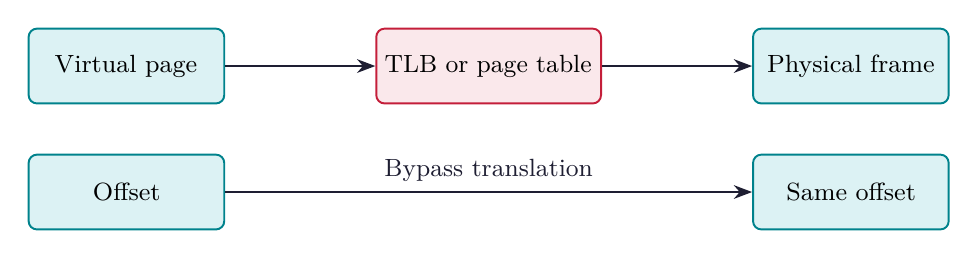
\begin{tikzpicture}[font=\small]
\node[block,text width=2.25cm] (v) at (0,0) {Virtual page};
\node[redblock,text width=2.62cm] (t) at (4.6,0) {TLB or page table};
\node[block,text width=2.25cm] (p) at (9.2,0) {Physical frame};
\node[block,text width=2.25cm] (o) at (0,-1.6) {Offset};
\node[block,text width=2.25cm] (z) at (9.2,-1.6) {Same offset};
\draw[arrow] (v.east)--(t.west);
\draw[arrow] (t.east)--(p.west);
\draw[arrow] (o.east)--(z.west) node[midway,above] {Bypass translation};
\end{tikzpicture}
\end{tcolorbox}

\subsection{TLB miss versus page fault}
\begin{enumerate}[leftmargin=*,itemsep=3pt]
\item \textbf{TLB hit.} The translation lookaside buffer (TLB) caches recent translations and access permissions. Check protection and form the physical address.
\item \textbf{TLB miss.} Walk the page table in hardware or software. If a usable entry exists, fill the TLB and continue. Main-memory residency is independent of whether the translation was cached.
\item \textbf{Page fault.} Trap to the operating system for a missing page, disallowed access or other fault condition. For a valid demand-page miss, obtain a frame, write a dirty victim if necessary, load or initialise the page, update mappings and restart the instruction. An illegal access may instead terminate the operation.
\item \textbf{Replacement and working set.} FIFO, LRU approximations and clock policies choose a victim. A working set is the group of actively used pages. If too few frames hold it, repeated faults can cause thrashing. Page replacement operates on main-memory frames, not CPU cache lines.
\end{enumerate}
\begin{tcolorbox}[examplebox,title={Translate an address and compute TLB timing}]
With $4\,\mathrm{KiB}$ pages, \texttt{0x12345} splits into VPN \texttt{0x12} and offset \texttt{0x345}. If that VPN maps to frame \texttt{0x2A}, the physical address is \texttt{0x2A345}.

Assume a serial 1 ns TLB lookup, 80 ns memory access, a one-access page-table walk, 98\% TLB hits and no page faults. A hit takes $81\,\mathrm{ns}$ and a miss $161\,\mathrm{ns}$. Mean access time is $0.98(81)+0.02(161)=82.6\,\mathrm{ns}$. Add a separate weighted fault-service cost only if the model specifies a page-fault probability.
\end{tcolorbox}

\begin{tcolorbox}[examplebox,title={Size a set-associative TLB tag}]
With 36-bit virtual byte addresses and $8\,\mathrm{KiB}$ pages, the offset is 13 bits and the VPN has 23 bits. A 128-entry four-way TLB has 32 sets, so the index takes five VPN bits. The virtual tag is $23-5=18$ bits, excluding any address-space identifier or page-size field. The physical frame number is stored data and does not contribute to this virtual tag length.
\end{tcolorbox}

\newpage
\begin{center}
  {\large\bfseries\color{myred} Quick Revision --- Module 5}\\[3pt]
  {\small\color{mydark} Memory Organisation and Virtual Memory $|$ EC502}
\end{center}
\noindent{\color{myred}\rule{\linewidth}{1.2pt}}
\begin{tcolorbox}[formulabox,title={Key Formulas at a Glance}]
\renewcommand{\arraystretch}{1.35}
\begin{tabularx}{\linewidth}{B{5.0cm}Y}
Chip capacity & $2^a$ words of $w$ bits equals $2^aw$ bits \\[3pt]
Cache sets & $S=C/(WB)$ for capacity $C$, block size $B$, and $W$ ways \\[3pt]
Cache fields & Offset $\log_2B$, index $\log_2 S$, remaining tag bits \\[3pt]
AMAT & Hit time plus miss rate times additional penalty \\[3pt]
Paging & Physical frame number concatenated with unchanged page offset \\[3pt]
\end{tabularx}
\end{tcolorbox}
\begin{tcolorbox}[defbox,title={One-Line Definitions}]
\textbf{Locality.} Tendency to reuse recent addresses or access nearby addresses.\par
\textbf{Associative memory.} Memory that finds entries matching a content key.\par
\textbf{TLB.} Fast cache of recent virtual-to-physical translations and permissions.\par
\end{tcolorbox}
\begin{tcolorbox}[exambox,title={Frequently Asked / Viva Questions}]
\begin{enumerate}[topsep=0pt, label=\textbf{Q\arabic*.}, itemsep=5pt]
\item \Q{Why does DRAM need refresh?}
Stored capacitor charge leaks.
\item \Q{Why is SRAM commonly used in processor caches?}
It has low latency and does not require refresh while powered.
\item \Q{What is the role of a cache tag?}
Identify the particular memory block occupying a line.
\item \Q{Can a direct-mapped cache choose among victims?}
No, each block has exactly one possible line.
\item \Q{What does a dirty bit say?}
The upper copy was modified and may need write-back.
\item \Q{Which miss remains when capacity and placement are unlimited?}
A first access still causes a compulsory miss.
\item \Q{Which cache mapping has zero index bits?}
Fully associative mapping has one set.
\item \Q{Does a TLB miss imply a page fault?}
No. A table walk may find a valid resident mapping.
\item \Q{What is unchanged by paging translation?}
The offset within the page or frame.
\item \Q{Why can thrashing reduce useful progress?}
Repeated page faults dominate execution time.
\end{enumerate}
\end{tcolorbox}
\begin{tcolorbox}[tikzbox,title={Summary comparison}]
\begin{tabularx}{\linewidth}{|B{4cm}|Y|}\hline
\textbf{Case} & \textbf{What to use} \\ \hline
SRAM / DRAM & Latch without refresh / capacitor storage with refresh. \\ \hline
Cache / virtual memory & Speed up block reuse / translate and protect address spaces. \\ \hline
TLB miss / page fault & Translation lookup refill / operating-system trap. \\ \hline
\end{tabularx}
\end{tcolorbox}

% -- Module 6 -----------------------------------------------------------------
\modulestart{6}{System Organisation and Input Output}

\section{System Organisation and Input Output}
\begin{tcolorbox}[defbox,title={I/O interface and controller}]
An input/output (I/O) controller connects a device to the computer interconnect. It buffers data, reports status, accepts commands and adapts timing or protocol. A device driver tells the controller which operations the operating system wants.
\end{tcolorbox}
\subsection{Buses, controller registers and addressing}
\begin{itemize}[leftmargin=*,itemsep=3pt]
\item \textbf{Interconnection.} A shared bus carries address, data and control. A bus master initiates a transaction, while the selected target responds. A bridge joins buses or translates protocols and address ranges.
\item \textbf{Registers.} Data registers or FIFOs hold transfers. Status registers expose ready, busy, done or error. Control registers configure the device, start operations or enable interrupts. Read or write side effects depend on the device.
\item \textbf{Memory-mapped I/O.} An address range is decoded to device registers. Loads and stores access it. Device regions need the appropriate memory attributes and ordering rules because caching or reordering can change peripheral effects.
\item \textbf{Isolated or port-mapped I/O.} A separate I/O address space and special instructions or transaction types select a port. It can preserve memory address space, but requires separate ISA or bus support.
\end{itemize}
\par\vspace{6pt}\noindent
\begin{tabularx}{\linewidth}{|B{2.6cm}|Y|Y|}\hline
Feature & Memory-mapped I/O & Port-mapped I/O \\ \hline
Address allocation & Uses part of the memory address space. & Uses a separate port address space. \\ \hline
Instruction & Ordinary loads and stores with device access semantics. & Dedicated port operations or a distinct bus cycle. \\ \hline
Addressing modes & Can use the load/store modes allowed for device memory. & Limited to the modes offered by the port instructions. \\ \hline
\end{tabularx}

\begin{tcolorbox}[tikzbox,title={CPU, main memory and the peripheral interface},unbreakable]
\centering
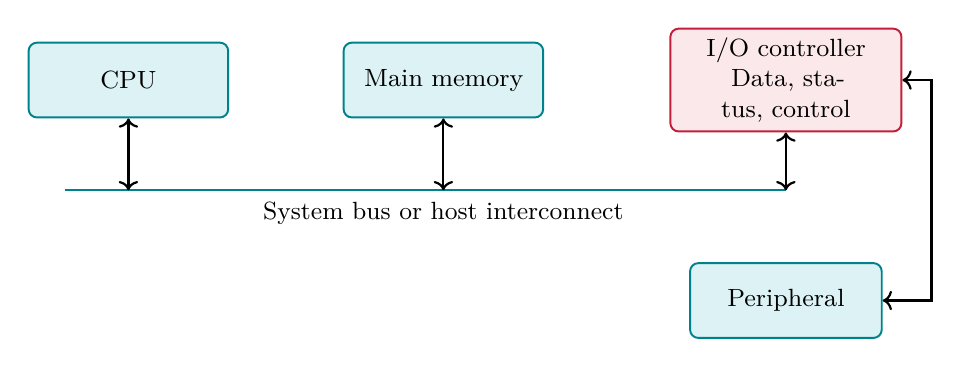
\begin{tikzpicture}[font=\small]
\node[block,text width=2.3cm] (cpu) at (0,0) {CPU};
\node[block,text width=2.3cm] (mem) at (4,0) {Main memory};
\node[redblock,text width=2.7cm] (ctl) at (8.35,0) {I/O controller\\Data, status, control};
\node[block,text width=2.2cm] (dev) at (8.35,-2.8) {Peripheral};
\draw[thick,myteal] (-.8,-1.4)--(8.35,-1.4);
\draw[<->,thick] (cpu.south)--(0,-1.4);
\draw[<->,thick] (mem.south)--(4,-1.4);
\draw[<->,thick] (ctl.south)--(8.35,-1.4);
\draw[<->,thick] (ctl.east)--(10.2,0)|-(dev.east);
\node[below] at (4,-1.42) {System bus or host interconnect};
\end{tikzpicture}
\end{tcolorbox}

\subsection{Synchronous and asynchronous transfer}
\begin{itemize}[leftmargin=*,itemsep=3pt]
\item \textbf{Synchronous bus.} Sender and receiver refer to agreed clock edges. An interface can add wait states until the target is ready. The shared protocol sets timing and direction for signals.
\item \textbf{Strobe.} A sender can assert data-valid without an acknowledgement if timing limits guarantee that the receiver can sample. This lacks explicit confirmation of completion.
\item \textbf{Handshaking.} A four-phase write starts when the source drives data and asserts request. The receiver latches stable data and asserts acknowledgement. The source deasserts request; the receiver then deasserts acknowledgement. This allows differing speeds. A practical clock-domain crossing needs appropriate synchronisation or an asynchronous FIFO.
\end{itemize}
\subsection{Arbitration}
When several masters request a shared bus, arbitration grants one at a time. In daisy-chain arbitration, a serial grant gives priority to the nearest requesting master. Parallel arbitration gives the arbiter separate requests and grants. Fixed priority can starve a low-priority master. Round robin rotates priority after service. Distributed arbitration lets contenders cooperate using a shared rule without one central grant controller.

\section{Programmed I/O and Interrupts}
\begin{tcolorbox}[defbox,title={Polling and interrupt}]
Polling asks the device repeatedly whether service is needed. An interrupt is a request that causes the CPU to suspend normal execution at an allowed point and transfer control to an interrupt service routine (ISR).
\end{tcolorbox}
\subsection{Programmed transfer and interrupt sequence}
\begin{enumerate}[leftmargin=*,itemsep=3pt]
\item \textbf{Programmed I/O.} The CPU issues a command, reads status until ready, and explicitly moves each item through a CPU register. Busy-waiting is simple but ties up the CPU.
\item \textbf{Interrupt request.} An enabled device raises a request. The interrupt controller may latch it and arbitrate priorities. The CPU accepts it at an architecture-defined point, usually an instruction boundary in a simple model.
\item \textbf{Enter ISR.} Save the return PC and required status. More registers may be saved by the ISR. In vectored I/O, a vector selects a handler or table entry. In a common-entry scheme, software polls pending status to identify the source.
\item \textbf{Complete service.} Read or write the controller, clear the cause and acknowledge completion where required. Restore state and execute interrupt return.
\end{enumerate}
\textbf{Priority and mask.} A mask controls which interrupts can be accepted. A non-maskable interrupt bypasses the ordinary mask for critical events. A priority controller may allow a higher-priority request to interrupt a lower-priority ISR. In a daisy-chained interrupt acknowledge, the first requesting device in the chain responds. A synchronous instruction exception is tied to the executing instruction, unlike an external device interrupt.

\begin{tcolorbox}[tikzbox,title={Daisy-chained interrupt acknowledgement},unbreakable]
\centering
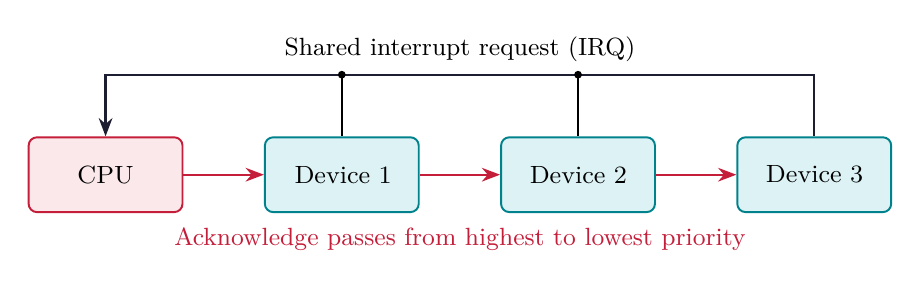
\begin{tikzpicture}[font=\small]
\node[redblock,text width=1.72cm] (cpu) at (0,0) {CPU};
\node[block,text width=1.72cm] (a) at (3.0,0) {Device 1};
\node[block,text width=1.72cm] (b) at (6.0,0) {Device 2};
\node[block,text width=1.72cm] (c) at (9.0,0) {Device 3};
\draw[redarrow] (cpu.east)--(a.west);
\draw[redarrow] (a.east)--(b.west);
\draw[redarrow] (b.east)--(c.west);
\draw[arrow] (c.north)--(9,1.27)--(0,1.27)--(cpu.north);
\draw[thick] (a.north)--(3,1.27) (b.north)--(6,1.27);
\fill (3,1.27) circle (1.4pt) (6,1.27) circle (1.4pt);
\node[above] at (4.5,1.31) {Shared interrupt request (IRQ)};
\node[below,myred] at (4.5,-.55) {Acknowledge passes from highest to lowest priority};
\end{tikzpicture}
\end{tcolorbox}

If Devices 2 and 3 request service together, Device 1 passes the acknowledgement along because it is idle. Device 2 claims it, supplies its vector and blocks the acknowledgement from Device 3. Device 3 can be serviced later. This fixes a physical priority order and can delay a device farther down the chain.

\begin{tcolorbox}[examplebox,title={Compare polling overhead with interrupt overhead}]
A 1 GHz CPU polls every $5\,\mu\mathrm s$ at 40 cycles per poll. Polling costs $200000(40)=8\times10^6$ cycles/s, or $0.8\%$ of CPU cycles. If the device instead interrupts at 4000 events/s with 300 cycles per service, cost is $1.2\times10^6$ cycles/s, or $0.12\%$. These estimates exclude common application processing. Polling response is bounded by the poll period in this simplified model. Interrupts have recognition and entry latency of their own.
\end{tcolorbox}

\section{Direct Memory Access}
\begin{tcolorbox}[defbox,title={Direct memory access}]
Direct memory access (DMA) transfers a block between a device and memory using a DMA-capable controller as bus master. The CPU sets up the transfer and handles completion, while the controller moves the data items.
\end{tcolorbox}
\begin{enumerate}[leftmargin=*,itemsep=3pt]
\item \textbf{Set up.} Driver supplies address or descriptors, length, direction and mode. A descriptor chain can describe multiple buffer segments.
\item \textbf{Request and grant.} Device or controller signals readiness. In a shared-bus model the DMA controller requests bus ownership and waits for a grant.
\item \textbf{Transfer.} DMA performs a device read plus memory write for input, or memory read plus device write for output, possibly as a direct combined transfer on suitable hardware. Update address and count after each unit.
\item \textbf{Finish.} Stop on terminal count or error, release bus ownership, and report status or interrupt the CPU. CPU and device must agree on when the buffer may be reused.
\end{enumerate}
\par\vspace{6pt}\noindent
\begin{tabularx}{\linewidth}{|B{3.05cm}|Y|Y|}\hline
Mode & Bus ownership & Typical trade-off \\ \hline
Burst & Controller holds bus for a block or bounded burst length. & Efficient block transfer, but CPU can wait longer for the bus. \\ \hline
Cycle stealing & Controller requests individual transfer cycles or small units. & Interleaves with CPU accesses while reducing available CPU bus cycles. \\ \hline
Transparent & Controller transfers only when the bus is otherwise idle. & Low CPU contention. Transfer completion time depends on idle availability. \\ \hline
\end{tabularx}

\begin{tcolorbox}[examplebox,title={DMA transfer time and contention}]
A $64\,\mathrm{KiB}$ block contains $16384$ 32-bit words. If the model completes one word per $20\,\mathrm{ns}$ bus cycle, data transfer takes $327.68\,\mu\mathrm s$. With $2\,\mu\mathrm s$ setup and no other stalls, total is $329.68\,\mu\mathrm s$. A single burst could occupy the bus for the data interval, while cycle stealing can spread bus use across time. It does not remove the number of data cycles needed.
\end{tcolorbox}

\textbf{Coherence and protection.} A DMA write changes memory and can leave a stale CPU cache copy. A DMA read can miss the latest dirty CPU data on a non-coherent system. Use platform-provided DMA synchronisation or hardware-coherent transfers. An I/O memory management unit (IOMMU) can translate permitted device addresses and constrain device access.

\section{Standard I/O Interfaces}
\begin{longtable}{|B{2.45cm}|>{\small\raggedright\arraybackslash}m{\dimexpr(\linewidth-2.45cm-6\tabcolsep-4\arrayrulewidth)/2\relax}|>{\small\raggedright\arraybackslash}m{\dimexpr(\linewidth-2.45cm-6\tabcolsep-4\arrayrulewidth)/2\relax}|}
\hline
Interface & Form and transaction model & Typical example \\ \hline
\endfirsthead
\hline
Interface & Form and transaction model & Typical example \\ \hline
\endhead
PCI & Conventional Peripheral Component Interconnect is a shared parallel expansion bus supporting configuration and bus mastering. & Legacy host expansion cards. \\ \hline
PCI Express & PCIe is a point-to-point serial packet interconnect. A root complex connects to endpoints directly or through switches. A link can contain multiple lanes. & Graphics cards, network adapters and NVMe storage. \\ \hline
USB & Universal Serial Bus is a host-controlled peripheral bus with hubs. The host enumerates devices, configures them and schedules transactions to endpoints. & Human interface devices, cameras and external storage. \\ \hline
SCSI / SATA & Small Computer System Interface (SCSI) defines a storage-oriented command model, historically used over parallel buses and now also carried over other transports. Serial ATA (SATA) is a point-to-point ATA storage link. & Disk and other storage connections. \\ \hline
RS-232 & Specifies electrical and interface signalling for serial equipment. A UART commonly supplies asynchronous start, data, optional parity and stop bits. A transceiver supplies the RS-232 electrical levels. & Serial terminals and instrumentation. \\ \hline
\end{longtable}

\textbf{USB transfer categories.} Control transfers configure devices and issue control requests. Bulk transfers move large reliable payloads without regular timing guarantees. Interrupt transfers get scheduled service opportunities for small periodic data, such as a keyboard. Isochronous transfers reserve periodic time for streams such as audio and do not retry missed packets at the transfer level. USB interrupt transfers are still scheduled by the host.

\newpage
\begin{center}
  {\large\bfseries\color{myred} Quick Revision --- Module 6}\\[3pt]
  {\small\color{mydark} System Organisation and Input Output $|$ EC502}
\end{center}
\noindent{\color{myred}\rule{\linewidth}{1.2pt}}
\begin{tcolorbox}[formulabox,title={Key Formulas at a Glance}]
\renewcommand{\arraystretch}{1.35}
\begin{tabularx}{\linewidth}{B{5.0cm}Y}
Polling demand & Poll frequency times cycles per poll \\[3pt]
Interrupt demand & Interrupts per second times cycles per service \\[3pt]
DMA data time & Transfer units times time per unit in a no-stall model \\[3pt]
Shared bus & Only the granted master initiates the shared transaction \\[3pt]
\end{tabularx}
\end{tcolorbox}
\begin{tcolorbox}[defbox,title={One-Line Definitions}]
\textbf{Interrupt vector.} Number or address used to select the corresponding handler.\par
\textbf{DMA.} Controller-driven data movement between memory and a device without a CPU copy per item.\par
\textbf{Handshaking.} Exchange of request and acknowledgement signals to coordinate a transfer.\par
\end{tcolorbox}
\begin{tcolorbox}[exambox,title={Frequently Asked / Viva Questions}]
\begin{enumerate}[topsep=0pt, label=\textbf{Q\arabic*.}, itemsep=5pt]
\item \Q{What is the difference between device status and control registers?}
Status reports controller state. Control registers configure or command it.
\item \Q{How does memory-mapped I/O select a device?}
Address decoding directs loads or stores to the device register range.
\item \Q{Why can synchronous buses still need wait states?}
A target may require extra cycles before data is ready.
\item \Q{What limits fixed-priority arbitration?}
Frequent high-priority requests can starve lower-priority masters.
\item \Q{How is a vector useful?}
It directs service to the appropriate ISR without searching every device.
\item \Q{Why does an ISR save state?}
Normal execution must resume with the required architectural state restored.
\item \Q{Does interrupt-driven I/O automatically imply DMA?}
No. An ISR can still move each item through a CPU register.
\item \Q{What is cycle stealing?}
DMA temporarily obtains a bus cycle or small group of cycles between other masters' accesses.
\item \Q{How do PCI and PCIe differ?}
Conventional PCI is a shared parallel bus. PCIe uses serial point-to-point links.
\item \Q{Which USB mode suits a real-time audio stream?}
Isochronous transfer, which provides periodic service opportunities.
\end{enumerate}
\end{tcolorbox}
\begin{tcolorbox}[tikzbox,title={Summary comparison}]
\begin{tabularx}{\linewidth}{|B{4cm}|Y|}\hline
\textbf{Case} & \textbf{What to use} \\ \hline
Polling & CPU waits or checks periodically, then moves data. \\ \hline
Interrupt-driven & Device requests CPU service when ready. CPU may still copy items. \\ \hline
DMA & CPU sets up a block transfer, and the controller moves the data. \\ \hline
\end{tabularx}
\end{tcolorbox}

% -- Module 7 -----------------------------------------------------------------
\modulestart{7}{Pipelining and Parallel Processing}

\section{Pipelining and Parallel Processing}
\begin{tcolorbox}[defbox,title={Parallelism and pipeline}]
Parallel processing uses overlapping or simultaneous operations to improve throughput or reduce time for a task. A pipeline splits work into stages and overlaps different items in different stages. Each item still traverses all stages it needs.
\end{tcolorbox}
\subsection{Pipeline stages, clock and speedup}
\begin{tcolorbox}[tikzbox,title={Classic five-stage instruction pipeline},unbreakable]
\centering
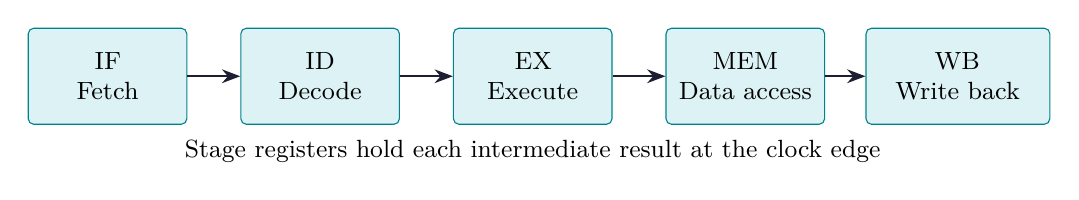
\begin{tikzpicture}[font=\small,stage/.style={draw=myteal,fill=hdrteal,rounded corners=2pt,text width=1.78cm,align=center,minimum height=1.22cm}]
\node[stage] (f) at (0,0) {IF\\Fetch};
\node[stage] (d) at (2.7,0) {ID\\Decode};
\node[stage] (e) at (5.4,0) {EX\\Execute};
\node[stage] (m) at (8.1,0) {MEM\\Data access};
\node[stage,text width=2.10cm] (w) at (10.8,0) {WB\\Write back};
\draw[arrow] (f.east)--(d.west);
\draw[arrow] (d.east)--(e.west);
\draw[arrow] (e.east)--(m.west);
\draw[arrow] (m.east)--(w.west);
\node[below] at (5.4,-.69) {Stage registers hold each intermediate result at the clock edge};
\end{tikzpicture}
\end{tcolorbox}

In a typical load/store design, IF reads the instruction, ID decodes and reads registers, EX calculates an ALU result or address, MEM accesses data for loads and stores, and WB writes a register when required. An arithmetic pipeline applies the same overlap to data operations, such as exponent comparison, alignment, significand addition, normalisation and rounding.
\begin{itemize}[leftmargin=*,itemsep=3pt]
\item \textbf{Clock period.} For logic delays $t_1,\ldots,t_k$ and stage-register overhead $t_r$, take $T_{\rm pipe}=\max_i t_i+t_r$. The longest stage sets the clock.
\item \textbf{Latency and throughput.} With $k$ cycles per item, one item takes $kT_{\rm pipe}$. For an ideal single-issue pipeline the steady completion rate is one item per cycle. Including fill and drain, $n$ items take $(k+n-1)T_{\rm pipe}$.
\item \textbf{Speedup.} If the nonpipelined reference runs each item in $\sum_i t_i$ without register overhead, speedup is $n\sum_i t_i/[(k+n-1)T_{\rm pipe}]$. For equal stage lengths and no overhead this becomes $kn/(k+n-1)$, approaching $k$ for large $n$.
\item \textbf{Efficiency.} Under the equal-stage ideal model, speedup divided by $k$ is $n/(k+n-1)$, the average fraction of occupied stage slots over the run. Count stalls separately if present.
\end{itemize}
\begin{tcolorbox}[examplebox,title={Unequal stages and finite workload}]
Four stage delays are $10,15,12,8\,\mathrm{ns}$ and each pipeline register adds $2\,\mathrm{ns}$. The pipeline clock is $17\,\mathrm{ns}$. For 20 items, nonpipelined time is $20(45)=900\,\mathrm{ns}$ and pipelined time is $(4+20-1)17=391\,\mathrm{ns}$, speedup $2.30$. One pipeline item takes $68\,\mathrm{ns}$ whereas one nonpipelined item takes $45\,\mathrm{ns}$. Overlap improves throughput even when single-item latency increases.
\end{tcolorbox}

\section{Pipeline Dependencies, Hazards and Control}
\begin{tcolorbox}[defbox,title={Pipeline hazard}]
A hazard is a condition that prevents an instruction from safely proceeding in its scheduled cycle. Resolve it by scheduling around it, forwarding an available value, stalling, or recovering from a wrong prediction.
\end{tcolorbox}
\par\vspace{6pt}\noindent
\begin{tabularx}{\linewidth}{|B{2.55cm}|Y|Y|}\hline
Hazard & Cause and example & Standard remedy \\ \hline
Structural & Two stages need the same resource in a cycle, such as instruction fetch and a load on one single-ported memory. & Arbitrate and stall, or use separate ports or instruction/data paths. \\ \hline
Data & An instruction reads a register before an earlier instruction's result is available (read after write, RAW). & Forward from a later stage when ready. Stall when the producer is still too late. \\ \hline
Control & The next PC depends on an unresolved branch or jump. & Wait, resolve early, or predict and flush wrong-path instructions on a miss. \\ \hline
\end{tabularx}

\subsection{RAW, WAR and WAW}
\begin{itemize}[leftmargin=*,itemsep=3pt]
\item \textbf{RAW, true dependence.} A consumer needs the value produced by an earlier instruction. A forwarding mux can route it from an execution or memory stage instead of waiting for register write-back.
\item \textbf{WAR, anti-dependence.} A younger write must wait until an older instruction has read the old value. \textbf{WAW, output dependence:} an older write must not replace a newer write to the same architectural register.
\item \textbf{When WAR and WAW matter.} Fixed in-order reads in ID and in-order writes in WB of a classic pipeline preserve order. Variable-latency or out-of-order execution may need register renaming to remove artificial name dependencies and ordered retirement to expose correct results.
\end{itemize}
\begin{tcolorbox}[examplebox,title={Load-use hazard with forwarding}]
Assume load data is ready at the end of MEM and ALU inputs are needed at the start of EX. The load's immediate consumer must stall one cycle. EX of SUB can receive ADD's ALU result by forwarding. A repeated stage label with an asterisk is a held or retried stage.
\par\vspace{6pt}\noindent
\begin{tabularx}{\linewidth}{|B{3.0cm}|*{8}{>{\centering\arraybackslash\small}X|}}\hline
Instruction & 1 & 2 & 3 & 4 & 5 & 6 & 7 & 8 \\ \hline
\texttt{LD R1,[R2]} & IF & ID & EX & MEM & WB & & & \\ \hline
\texttt{ADD R3,R1,R4} & & IF & ID & ID$^*$ & EX & MEM & WB & \\ \hline
\texttt{SUB R5,R3,R6} & & & IF & IF$^*$ & ID & EX & MEM & WB \\ \hline
\end{tabularx}

The hazard unit freezes the PC and the fetch/decode register for one cycle and inserts a bubble into EX in cycle 4. The load advances to MEM and its data forwards to ADD in cycle 5.
\end{tcolorbox}

\subsection{Branch control and effective CPI}
For a resolved or correctly predicted next PC, fetching can continue. On misprediction, redirect fetch and flush the younger wrong-path instructions before they change architectural state. The branch penalty depends on the resolution stage and fetch logic.
\begin{tcolorbox}[examplebox,title={Sum independent stall contributions}]
Assume base CPI 1. If $25\%$ of instructions are loads and $20\%$ of those loads have an immediate use costing one stall, the load contribution is $0.25(0.20)(1)=0.05$. If $18\%$ of instructions are branches, $10\%$ of branches are mispredicted and each costs 3 cycles, the branch contribution is $0.18(0.10)(3)=0.054$. Ignoring overlap and other stalls, effective CPI is $1.104$. Multiply this by instruction count and clock period to find CPU time.
\end{tcolorbox}

\section{Forms of Parallel Processing}
\subsection{Flynn's classification}
Classify by how many instruction and data streams are active. Streams describe logical execution, not the number of pipeline stages.
\par\vspace{6pt}\noindent
\begin{tabularx}{\linewidth}{|B{2.3cm}|Y|Y|}\hline
Class & Streams & Representative organisation \\ \hline
SISD & Single instruction, single data & Conventional single instruction stream over one data stream. It can still use a pipeline internally. \\ \hline
SIMD & Single instruction, multiple data & One operation controls several data lanes. Vector instructions and array processors are common examples. \\ \hline
MISD & Multiple instruction, single data & Different processing operations on the same logical data stream. Uncommon as a general-purpose organisation. \\ \hline
MIMD & Multiple instruction, multiple data & Independent instruction streams on separate cores or nodes. \\ \hline
\end{tabularx}

\begin{itemize}[leftmargin=*,itemsep=4pt]
\item \textbf{Instruction-level parallelism.} Pipelining overlaps instructions. A superscalar CPU can start more than one independent instruction per cycle. Dependencies and available issue units limit useful overlap.
\item \textbf{Very long instruction word (VLIW).} The compiler schedules independent operations into explicit bundles for several units. This can simplify issue hardware. Code scheduled for a particular bundle format or timing model may need recompilation for another implementation.
\item \textbf{Data-level parallelism.} A vector processor applies vector instructions to elements through vector lanes or pipelines. An array processor uses a collection of processing elements controlled together. Both exploit repeated operations over elements.
\item \textbf{Task or thread parallelism.} Separate tasks or threads run on multiple cores. A shared-memory multiprocessor gives processors a common address space. A distributed-memory multicomputer uses private memory per node and exchanges messages.
\item \textbf{Shared memory variants.} Uniform memory access (UMA) abstracts similar memory access cost across processors. Non-uniform memory access (NUMA) has different local and remote costs. Both may still expose one address space.
\end{itemize}
\subsection{Synchronization, coherence and speedup limits}
\begin{itemize}[leftmargin=*,itemsep=3pt]
\item \textbf{Race.} Two cores reading the same counter and independently writing back incremented values can lose an update. Protect the critical section with a lock built on atomic operations, or use atomic increment where suitable.
\item \textbf{Barrier.} Workers finish their current phase before any proceeds to the next. In a message-passing system, explicit sends and receives communicate data and coordinate dependencies.
\item \textbf{Coherence and ordering.} Coherence governs observations of writes to a single address across caches. Memory consistency specifies allowed orderings across accesses, including different addresses. Use the synchronization primitives defined by the programming model.
\item \textbf{Speedup limit.} If a serial fraction $f_s$ remains, ideal speedup on $p$ workers is $1/[f_s+(1-f_s)/p]$. With $f_s=0.10$ and eight workers, it is $4.71$, even before communication, imbalance and synchronization costs.
\end{itemize}
\begin{tcolorbox}[examplebox,title={Follow a coherence invalidation}]
Both cores cache a line holding $X=0$. When core A requests write ownership to store 1, an invalidation protocol invalidates core B's shared copy before granting exclusive write permission. After a properly synchronised handoff, core B's next load can obtain the updated value from the owner or coherent memory system. A shared writable region can instead be mapped uncached on a suitable system, using the platform's ordering rules, at the cost of extra memory traffic. A lock or barrier also supplies ordering, but does not by itself repair stale cache data on a non-coherent system.
\end{tcolorbox}

% Keep the heading and definition together where the preceding box ends low on a page.
\par
\ifdim\dimexpr\pagegoal-\pagetotal\relax<108pt\relax
  \newpage
\fi
\section{Interconnection Networks}
\begin{tcolorbox}[defbox,title={Interconnect}]
An interconnection network carries requests and responses among processors, memories and I/O endpoints. Topology says which links exist. Routing chooses a path, and flow control manages use of links and buffers.
\end{tcolorbox}
\par\vspace{6pt}\noindent
\begin{tabularx}{\linewidth}{|B{2.8cm}|Y|Y|}\hline
Topology & Paths & Main cost or limitation \\ \hline
Bus & One shared communication medium. & Low wiring cost. Arbitration and shared bandwidth limit scaling. \\ \hline
Ring & Nodes connect to neighbours in a loop. & Small node degree. Messages may traverse several hops. \\ \hline
Mesh & Nodes connect to nearby grid neighbours. & Regular wiring. Distant communication takes multiple hops. \\ \hline
Crossbar & Crosspoints connect each input to each output. & Nonblocking for connections to distinct outputs. An $N$ by $N$ crossbar needs $N^2$ crosspoints. \\ \hline
Omega network & $\log_2 N$ stages of $2$ by $2$ switches with shuffle links for $N=2^k$. & Uses $(N/2)\log_2N$ switches, but internal conflicts can block distinct-output routes. \\ \hline
\end{tabularx}

\begin{tcolorbox}[tikzbox,title={Crossbar example: concurrent requests to different outputs},unbreakable]
\centering
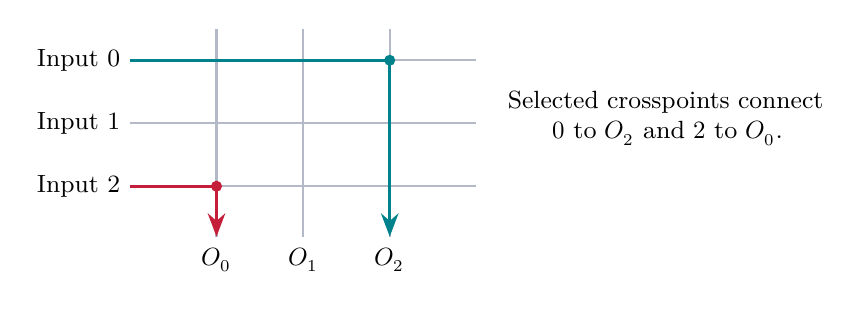
\begin{tikzpicture}[font=\small,x=1.1cm,y=.8cm]
\foreach \i in {0,1,2}{
 \draw[mgframe,thick] (0,2-\i)--(4,2-\i);
 \node[left] at (0,2-\i) {Input \i};
 \draw[mgframe,thick] (1+\i,2.5)--(1+\i,-.8);
 \node[below] at (1+\i,-.82) {$O_{\i}$};
}
\draw[myteal,very thick,-Stealth] (0,2)--(3,2)--(3,-.8);
\draw[myred,very thick,-Stealth] (0,0)--(1,0)--(1,-.8);
\fill[myteal] (3,2) circle (2pt);
\fill[myred] (1,0) circle (2pt);
\node[align=center,text width=4cm,anchor=west] at (4.25,1.08) {Selected crosspoints connect $0$ to $O_2$ and $2$ to $O_0$.};
\end{tikzpicture}
\end{tcolorbox}
\subsection{A multistage routing example}
In an eight-input Omega convention in which adjacent inputs share the first switch, successive destination bits choose the upper or lower output link at each stage, most significant first. The interstage shuffle permutes link positions. There are $3$ stages of $4$ switches, or 12 switches total. Input 0 to destination \texttt{000} and input 1 to destination \texttt{001} need the same upper output of their first switch because both destination high bits are 0. They can contend even though their final outputs differ. In a crossbar the two distinct outputs could be selected concurrently. Evaluate networks by switch/wire cost, latency, bandwidth, blocking and scalability.

\newpage
\begin{center}
  {\large\bfseries\color{myred} Quick Revision --- Module 7}\\[3pt]
  {\small\color{mydark} Pipelining and Parallel Processing $|$ EC502}
\end{center}
\noindent{\color{myred}\rule{\linewidth}{1.2pt}}
\begin{tcolorbox}[formulabox,title={Key Formulas at a Glance}]
\renewcommand{\arraystretch}{1.35}
\begin{tabularx}{\linewidth}{B{5.0cm}Y}
Ideal pipeline time & $(k+n-1)T_{\rm pipe}$ for $n$ items and $k$ stages \\[3pt]
Pipeline period & $\max_i(t_i)+t_r$ \\[3pt]
Effective CPI & Base CPI plus weighted stall cycles per instruction \\[3pt]
Parallel speedup & $1/[f_s+(1-f_s)/p]$ under ideal workload split \\[3pt]
Omega switch count & $(N/2)\log_2 N$ for a power-of-two port count \\[3pt]
\end{tabularx}
\end{tcolorbox}
\begin{tcolorbox}[defbox,title={One-Line Definitions}]
\textbf{Forwarding.} Route a ready result directly to a later consumer stage.\par
\textbf{Bubble.} Empty or invalid pipeline slot that makes no architectural update.\par
\textbf{Array processor.} Multiple processing elements operated together on different data.\par
\end{tcolorbox}
\begin{tcolorbox}[exambox,title={Frequently Asked / Viva Questions}]
\begin{enumerate}[topsep=0pt, label=\textbf{Q\arabic*.}, itemsep=5pt]
\item \Q{Does a pipeline necessarily reduce one instruction's latency?}
No. Its main benefit is overlapping work to raise throughput.
\item \Q{What sets the pipeline clock period?}
The slowest stage plus register overhead.
\item \Q{When does load-use still stall with forwarding?}
When load data becomes available after the dependent instruction needs it.
\item \Q{What is a structural hazard?}
Multiple operations request an insufficiently replicated resource at the same time.
\item \Q{Are WAR and WAW true value dependencies?}
No. They arise from reuse of a destination name.
\item \Q{What happens on a branch misprediction?}
Wrong-path work is flushed and fetch restarts at the correct PC.
\item \Q{How do vector and array processors exploit data parallelism?}
Vector instructions operate on sequences using lanes or pipelines. Array processors use multiple controlled processing elements.
\item \Q{What defines MIMD?}
Multiple instruction streams operating on multiple data streams.
\item \Q{Why use a barrier?}
No worker in the next phase proceeds until participating workers finish the current phase.
\item \Q{Why can a multistage network block two distinct destinations?}
Both paths may require the same internal link.
\end{enumerate}
\end{tcolorbox}
\begin{tcolorbox}[tikzbox,title={Summary comparison}]
\begin{tabularx}{\linewidth}{|B{4cm}|Y|}\hline
\textbf{Case} & \textbf{What to use} \\ \hline
Pipelining & Overlap stages of different work items. \\ \hline
SIMD / MIMD & Shared operation on several data items / independent instruction streams. \\ \hline
Crossbar / Omega & More crosspoints with flexible distinct-output paths / fewer switches with possible internal contention. \\ \hline
\end{tabularx}
\end{tcolorbox}

\end{document}
